% From OUP/Overleaf for Genetics, modified by Nilo Merino Recalde:
% https://github.com/nilomr

\documentclass[9pt, onecolumn, twoside, lineno]{gsajnl}
% Use the documentclass option 'lineno' to view line numbers, and twocolumn to have two columns obviously

\usepackage{epstopdf}
\usepackage{orcidlink}
\usepackage{caption}
\usepackage{tipa}
\usepackage{doi}
\usepackage{tabularray}
\usepackage{tcolorbox}
\usepackage{hyperref}



\usepackage{setspace}
\setstretch{1.15} % body line space
%\renewcommand{\familydefault}{\sfdefault} % sans serif for review

\runningauthor{Merino Recalde \textit{et al}., 2024 }
\runningtitle{The demographic drivers of cultural evolution in bird song}

\begin{document}

\title{A multilevel study of the demographic drivers of cultural evolution in bird song}
\author[1,$\ast$]{Nilo Merino Recalde\,\orcidlink{0000-0003-3903-1288}} 
\author[1]{Andrea Estandía\,\orcidlink{0000-0002-3895-2141}}
\author[1,2]{Sara C. Keen\,\orcidlink{0000-0002-2988-8280}}
\author[1]{Ella F. Cole\,\orcidlink{0000-0002-2689-946X}} 
\author[1]{Ben C. Sheldon\,\orcidlink{0000-0002-5240-7828}} 

\affil[1]{
    Edward Grey Institute, Department of Biology, University of Oxford, Oxford, UK
}
\affil[2]{
    Earth Species Project, 1536 Oxford St. Berkeley CA 94709, US
}


\correspondingauthoraffiliation[$\ast$]{Corresponding author: \href{mailto:nilo.recalde@biology.ox.ac.uk}{nilo.recalde@biology.ox.ac.uk}}

\begin{abstract}
Social learning within communities can lead to shared behavioural patterns that persist over time, which we know as culture. Examples of culture include bird and whale songs, cetacean feeding techniques, and avian and mammalian migratory routes. Shaped by neutral and selective forces, animal cultures evolve dynamically and form cultural traditions that vary greatly in their diversity and stability. These cultural traits can influence individual and group survival, population structure, and even inform conservation efforts, underscoring the importance of understanding how population processes interact with social learning to shape culture. Although the impact of social learning mechanisms and biases has been extensively explored, the role of demographic factors---such as population turnover, immigration, and age structure---on cultural evolution has received theoretical attention but rarely been subject to empirical investigation in natural populations. Doing so requires very complete trait sampling and detailed individual life history data, which are hard to acquire in combination. To this end, we compiled a multi-generational dataset containing over 109,000 songs from >400 repertoires in a population of great tits (\textit{Parus major}), trained a deep metric learning model to re-identify individuals and quantify song similarity, and fit spatially explicit regression models of cultural diversity and turnover at the individual and neighbourhood scales. We show that demographic variation within the small spatial scales at which learning takes place has the potential to impact the diversity and pace of change of animal vocal cultures. In particular, longer natal dispersal distances within the population reduce cultural diversity and uniqueness, while immigrant birds seem to acquire local song types rather than introducing new ones, but tend to have larger repertoires and so increase the absolute diversity of neighbourhoods. Birds of the same age tend to have more similar repertoires, and neighbourhoods comprising a mix of ages tend to have more cultural diversity. Individual turnover is the primary driver of cultural change. However, several factors slow this change: dispersal, a higher proportion of immigrant birds, and an older population. Our analyses support theoretical expectations regarding a key role of demographic processes in cultural evolution, while highlighting their interaction with species-specific factors such as the timing of song acquisition.
\end{abstract}

\maketitle
\vspace{-13pt}% Only used for adjusting extra space in the left column of the first page

\section{Results and Discussion}

\lettrine[lines=2]Some behavioural traits are shared and persist within communities due to social learning \autocite{viciana2021}. We refer to these behaviours as 'animal culture', exemplified by tool use in capuchin monkeys \autocite{falotico2019}, the learned songs of oscine birds \autocite{aplin2017, riebel2015, williams2021}, migration routes \autocite{jesmer2018, berdahl2018, byholm2022}, and the feeding techniques of some cetaceans \autocite{allen2013, rendell2001}. Animal cultures are not static: neutral and selective mechanisms influence the frequency of cultural traits \autocite{potvin2015, williams2021}, leading to a process of cultural evolution. The resulting cultural traditions differ considerably in their diversity and stability \autocite{tchernichovski2017}, determined by both learning biases and mechanisms and the demographic structure of populations \autocite{deffner2022a, kandler2017}. 

While the role of social learning strategies and biases---frequency dependence, tutor biases, etc.---has been extensively studied \autocite{pike2010, kendal2015, aplin2017, lachlan2018, tchernichovski2021}, there exists a substantial gap in our understanding of how demography contributes to the emergence and persistence of distinct cultural traits within wild populations. Processes such as the recruitment of juveniles, immigration, emigration, mortality, and variation in age structure are likely to strongly affect an individual's opportunities for learning and exposure to different cultural variants, which has been amply emphasized by theoretical work \autocite{deffner2022a, deffner2022, kandler2023, fogarty2019, deffner2020, derex2016, kirby2021, nunn2009, barta2023, dyble2024, chimento2024}. However, translating theoretical expectations into empirical evidence remains a challenge (see \autocite{chimento2021, fayet2014, payne1993} for exceptions).


\begin{figure*}[!ht]
    \centering
    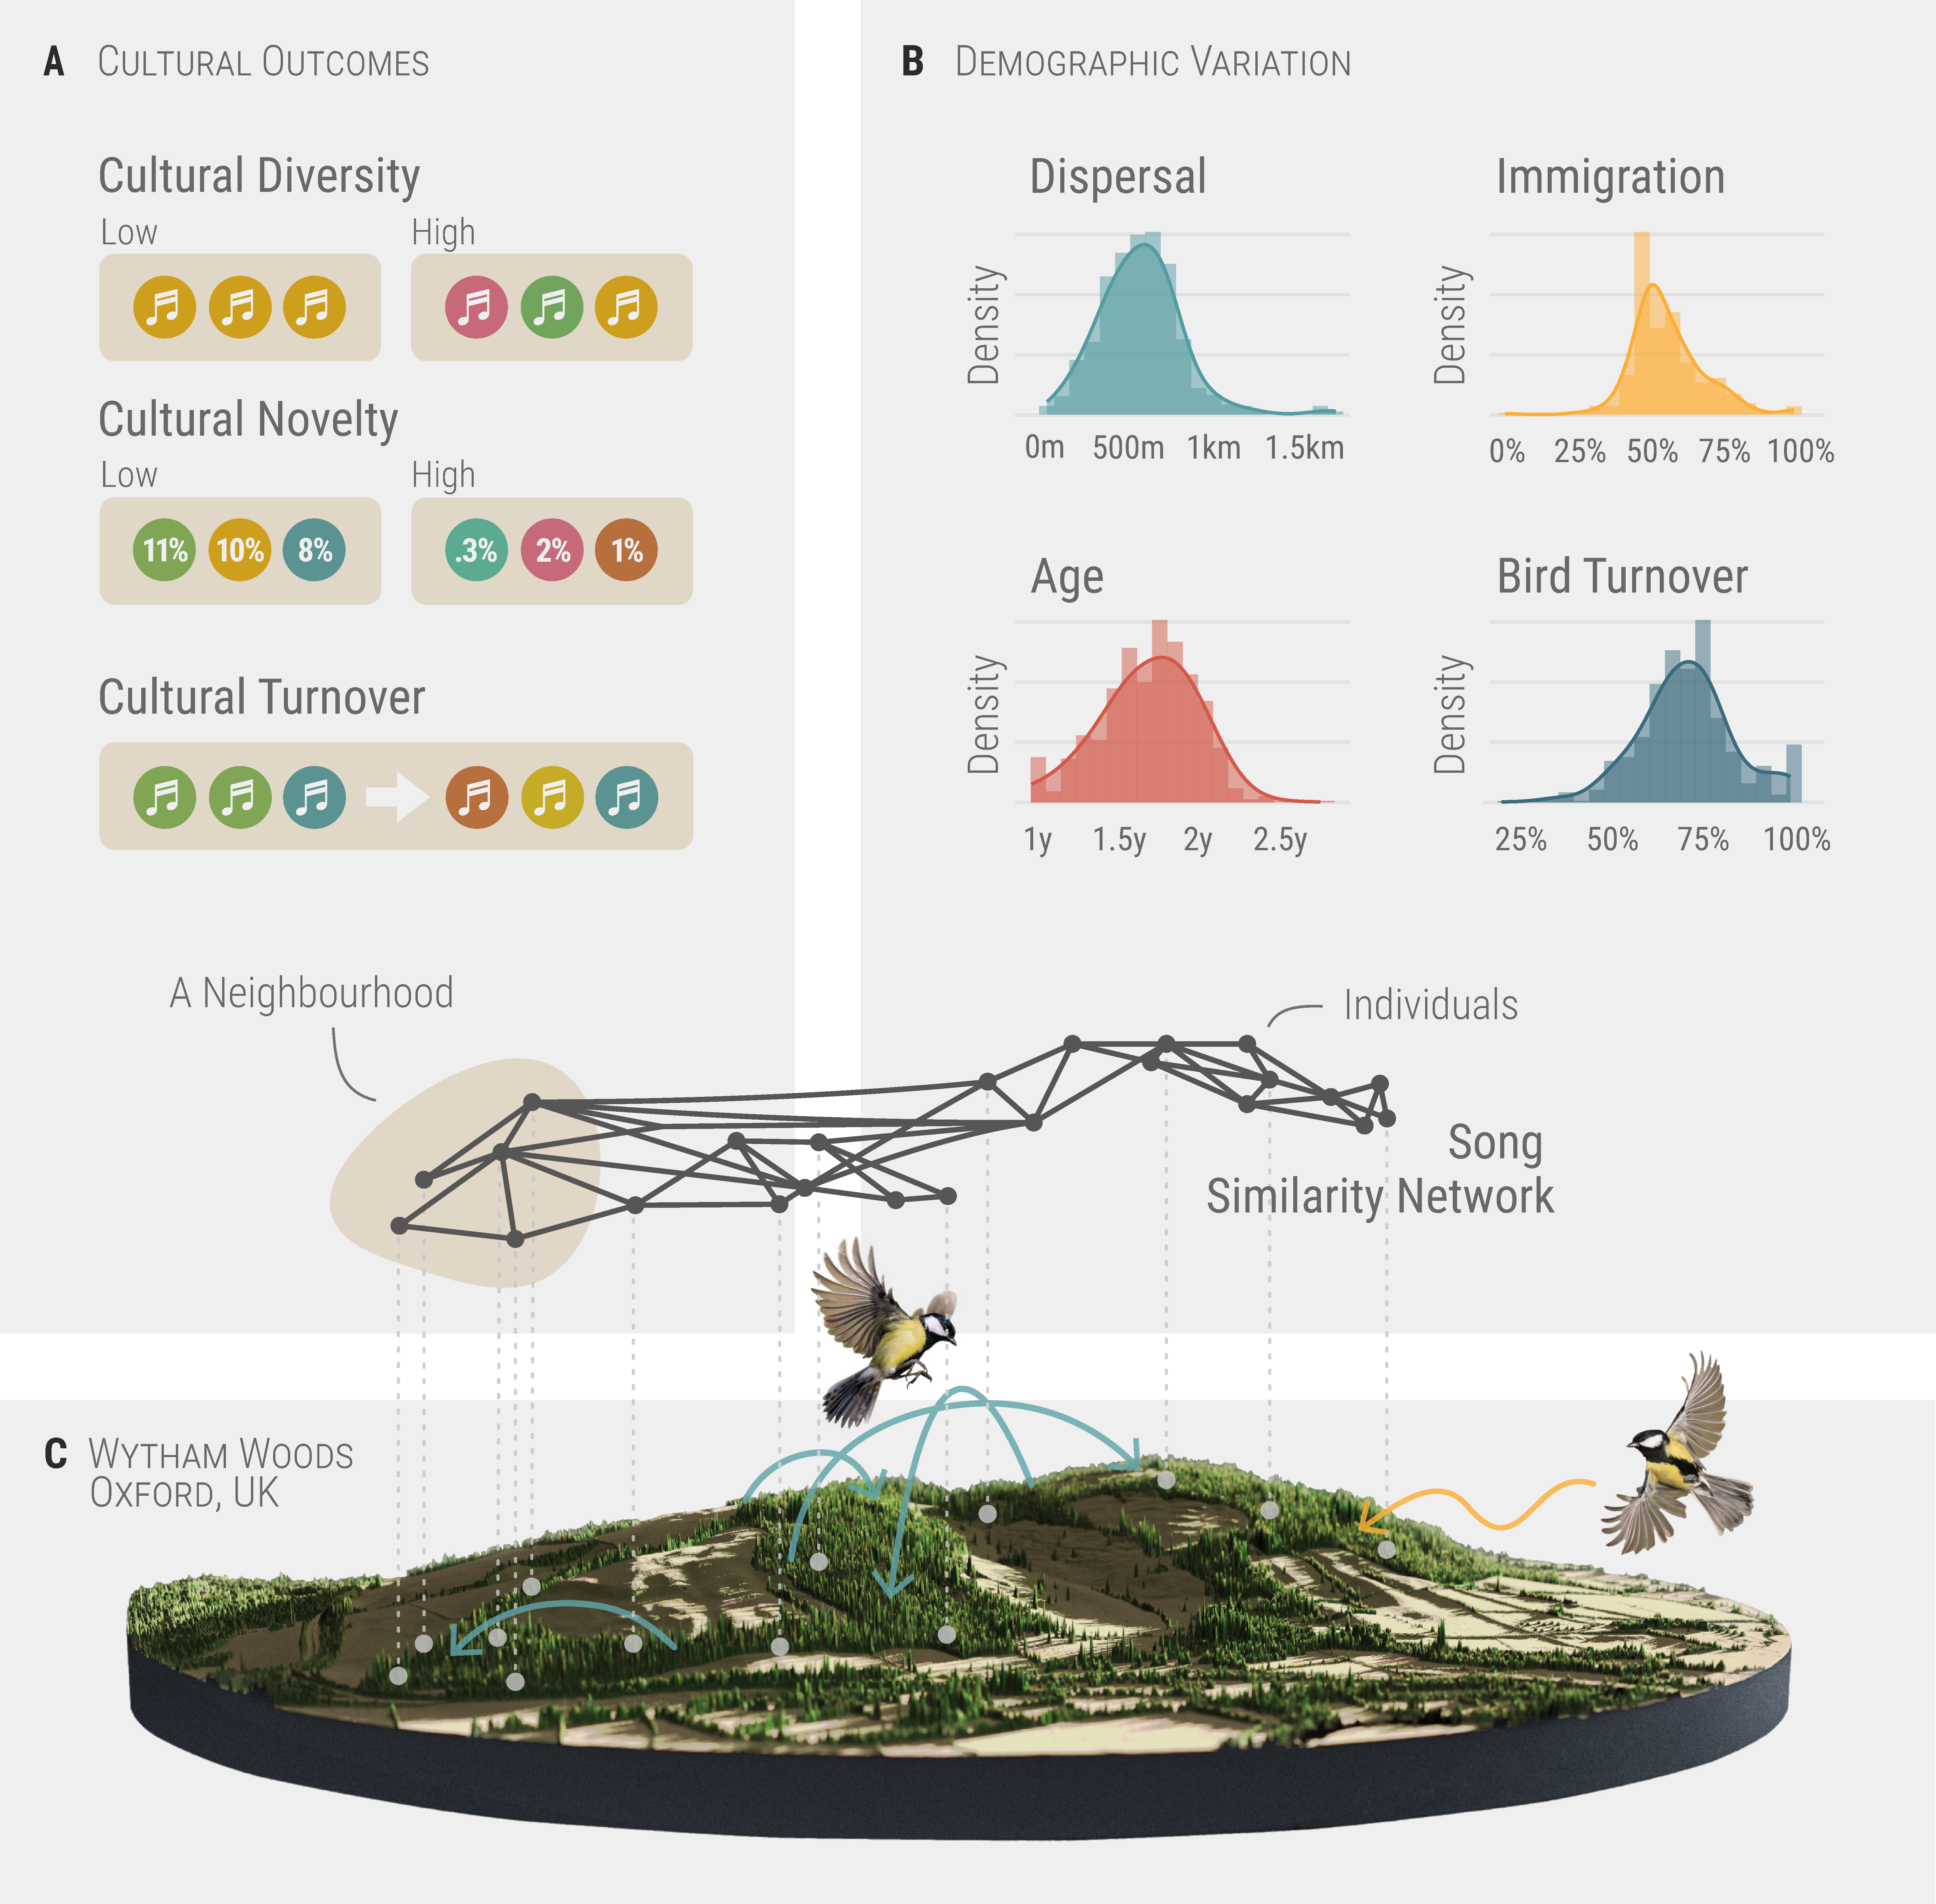
\includegraphics[width=\linewidth]{figures/chapter_4/FIG1.pdf}
    \mycaption{Study system and main variables in our analysis}{
        (A) Cultural variables measured at the neighbourhood level. Higher values of cultural diversity indicate that there are more different song types in the neighbourhood relative to the total song output. Higher cultural uniqueness indicates that the songs in the neighbourhood are on average less common in the population, and higher cultural turnover indicates that the neighbourhood's song repertoire has changed more from one year to the next. See \hyperref[sc:op-definitions]{definitions} for full definitions.

        (B) Variation in the demographic properties and composition of neighbourhoods across the population. See \hyperref[sc:group-properties]{demographic variables} for full definitions.

        (C) Cartoon representation of the pairwise continuous repertoire similarity network used in our individual level analyses. Each node represents an individual bird, and the edges represent the similarity between their song repertoires. The network is based on the similarity of the songs produced by each bird during the dawn chorus, and is used to estimate the cultural similarity between individuals.
        
        (D) 3D render of our study site, Wytham Woods, seen from the East. Image based on first return LiDAR data \autocite{defra2020} and made with rayshader \autocite{rayshader2023}. Elevation is exaggerated. Aquamarine (darker) arrows represent natal dispersal within the population, and the yellow (lighter) arrow represents immigration into the population, two of the variables used in this work. Age and bird (individual) turnover are not depicted.        
    }
    \label{c4_fig:main}
\end{figure*}

Culture is increasingly recognized as both a fundamental aspect of many animals' lives and a valuable tool in monitoring and conservation efforts \autocite{brakes2019, brakes2021}. Cultural traits play a role in the survival and reproduction of individuals and social groups; they reflect or even shape the structure of the population \autocite{brakes2019}, and can be lost when habitat fragmentation and population decline lead to reduced learning opportunities \autocite{paxton2019, crates2021}. A comprehensive understanding of cultural change and loss, then, requires that we have the ability to detect and study not just intrinsic factors---social, cultural, cognitive---but also extrinsic, ecological and demographic processes. This entails identifying the relevant spatial and temporal scales at which these processes manifest within natural populations, as well as their relative importance. 

To contribute to this goal, we built a comprehensive dataset that spans three years and documents the dawn songs produced by male great tit birds during 454 breeding attempts in a single population located in Wytham Woods, UK. The population's marked variation in individual turnover, postnatal dispersal distances, age structure, and immigration across space---known through ongoing long-term monitoring \autocite{lack1964}---allowed us to estimate their effects on song cultural repertoires at both individual and group levels. First, we assigned more than 109,000 songs in 330 song repertoires to 242 individual birds through a combination of direct physical capture, radio frequency identification microchips, and a novel song-based re-identification method using a deep metric learning model. Then, we quantified individual and group-level traits and analysed variation in song cultural similarity, diversity, and turnover (see \hyperref[sc:group-properties]{definitions}) using network and spatially explicit Bayesian multilevel regression models. See \autoref{c4_fig:main} for a visual abstract of the study.


\begin{figure*}[!hbt]
    \centering
    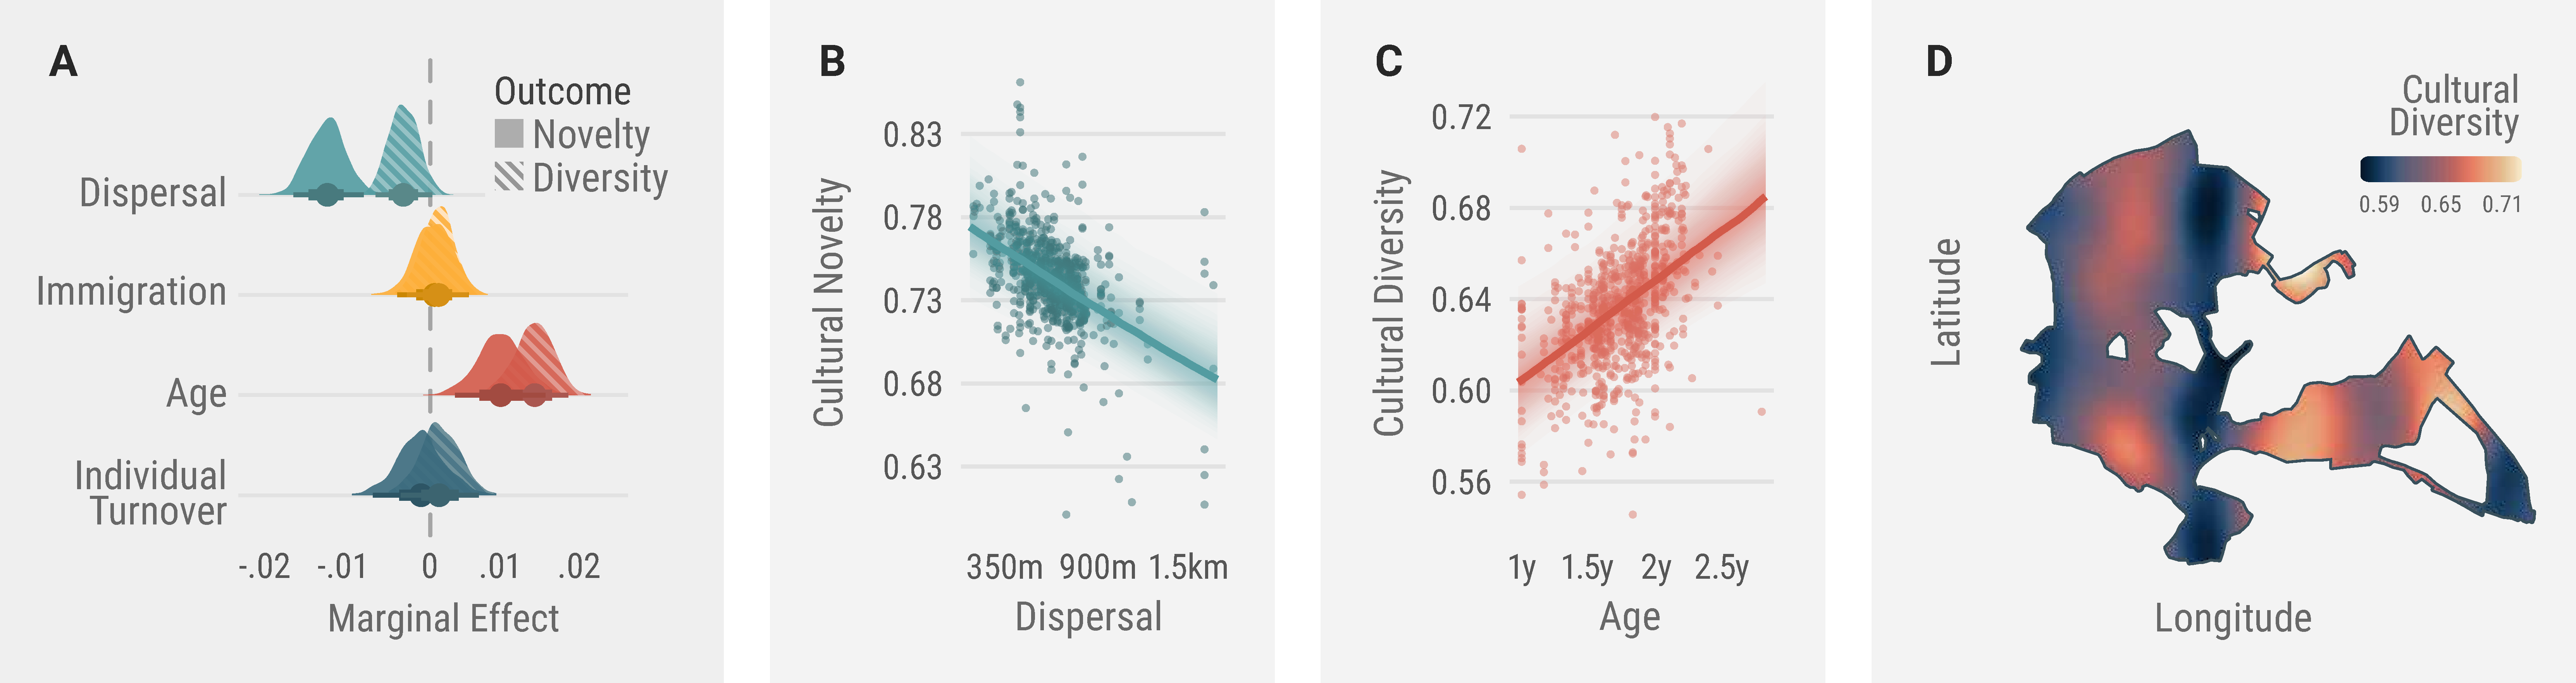
\includegraphics[width=\linewidth]{figures/chapter_4/FIG3.pdf}
    \mycaption{Influence of demographic variables on cultural diversity and uniqueness within neighbourhoods}{
        (A) Marginal effects at the mean of neighbourhood characteristics including mean dispersal distance, proportion of immigrant birds, average age, and individual turnover. See \hyperref[sc:group-properties]{methods} for full definitions.
        (B) Adjusted predictions and partial residuals of the effect of mean neighbourhood dispersal distance on cultural uniqueness. Low-dispersal neighbourhoods are those in which birds were born in the same area.
        (C) Adjusted predictions and partial residuals of the effect of the mean age of the neighbourhood on cultural diversity. A neighbourhood with a mean age of 1 would be one where all birds are breeding for the first time.
        (D) The average distribution of cultural diversity in the population across space during the study period (2020-2022). This map captures the residual variation in cultural diversity after taking into account the demographic variables in (A). The map is based on a Gaussian process model with an exponentiated-quadratic kernel covariance function, which allows us to interpolate between the locations where we have data.
    }
    \label{c4_fig:diversity}
\end{figure*}

Our results reveal an interplay of demographics and song cultural dynamics that, albeit complex, largely matches theoretical expectations, as discussed below. This work also demonstrates that bird song, which already provides what is perhaps the largest body of evidence for cultural change in animals \autocite{laland2006}, also has the potential to help us shed light on the impact of other population processes on animal cultures, owing to the fact that we can sample individual song repertoires with relative ease.

\subsection{Reduced dispersal, higher immigration and and age associated with higher cultural diversity}

Population genetics provides robust evidence supporting the notion that high dispersal rates facilitate gene flow, which, in turn, reduces the efficacy of selection and diversification. Conversely, low dispersal facilitates genetic differentiation through mechanisms such as mutation and drift, leading to allopatric population divergence \autocite{suarez2022, claramunt2011, papadopoulou2009}. Were we to adhere to an analogy from genetics to culture, we would anticipate that reduced dispersal rates will decelerate the diffusion of cultural traits \autocite{nunn2009}. This, in turn, should result in the maintenance of distinct behavioural patterns within populations if learning is somewhat accurate, leading to a greater number of cultural variants unique to a neighbourhood or region \autocite{whitehead2012, planque2014}. Our analysis indeed indicates that neighbourhoods (see \hyperref{sc:group-properties}{definitions} where more birds have remained in proximity to their natal areas harbour greater and more unique cultural diversity (\textit{diversity:} $P(\beta_{disp (\overline{m})} < 0 | D) = 1,~ mem = -0.018,~CI_{95\%}~[-0.023, -0.012]$; \textit{uniqueness:} $P(\beta_{disp (\overline{m})} < 0 | D) = 0.96,~ mem = -0.005,~CI_{95\%}~[-0.01, 0]$; \figref[a\&b]{c4_fig:diversity}, \autoref{table:model_estimates}; see \autoref{sc:group-properties}), in line with prior research at a much coarser grain \autocite{fayet2014}. 

The analogy breaks down as soon as we consider the underlying individual-level mechanisms, however, due to complex interactions between the timing of dispersal and learning mechanisms that are specific to the cultural domain. Some species only learn songs from their parents and early in life, in a manner reminiscent of genetic inheritance, while others learn continuously from their neighbours, or only after dispersal (see \autocite{searcy2021} for an overview of different strategies). In the case of our study species, the great tit, these learning mechanisms are thought to involve selective retention or modification of songs encountered early in life, while they disperse, and up until before they begin breeding for the first time---a process that results in crystallized repertoires of 1 to $\simeq$ 10 different song types \autocite{mcgregor1982b,rivera-gutierrez2011,merinorecalde2023a}. In our individual-level analysis, we see that birds that dispersed over longer distances tend to have learned repertoires composed of songs that are more common within the population (\textit{uniqueness:} $P(\beta_{disp (m)} < 0 | D) = 1,~mem = -0.2,~CI_{95\%}~[-0.3, -0.09]$; \figref[b]{c4_fig:individual}, \autoref{table:model_estimates}), and possibly smaller repertoires as well (\textit{rep.size:} $P(\beta_{disp (m)} < 0 | D) = 0.91,~mem = -0.2,~CI_{95\%}~[-0.44, 0.05]$; \figref[b]{c4_fig:individual}; \autoref{table:model_estimates}). We hypothesize that birds with more extensive movements are more likely to sample and acquire a larger proportion of common cultural variants, simply because they are exposed to more songs across their learning period. This finds support in a spatially explicit simulation of song learning with dispersal, which shows this pattern would emerge under positively frequency-dependent learning or a process leading to similar acquisition curves (see \autoref{fig:supp_dispersal_simulation}; note that we do not currently know which learning strategies are employed by great tits).

\begin{figure*}[!t]
    \centering
    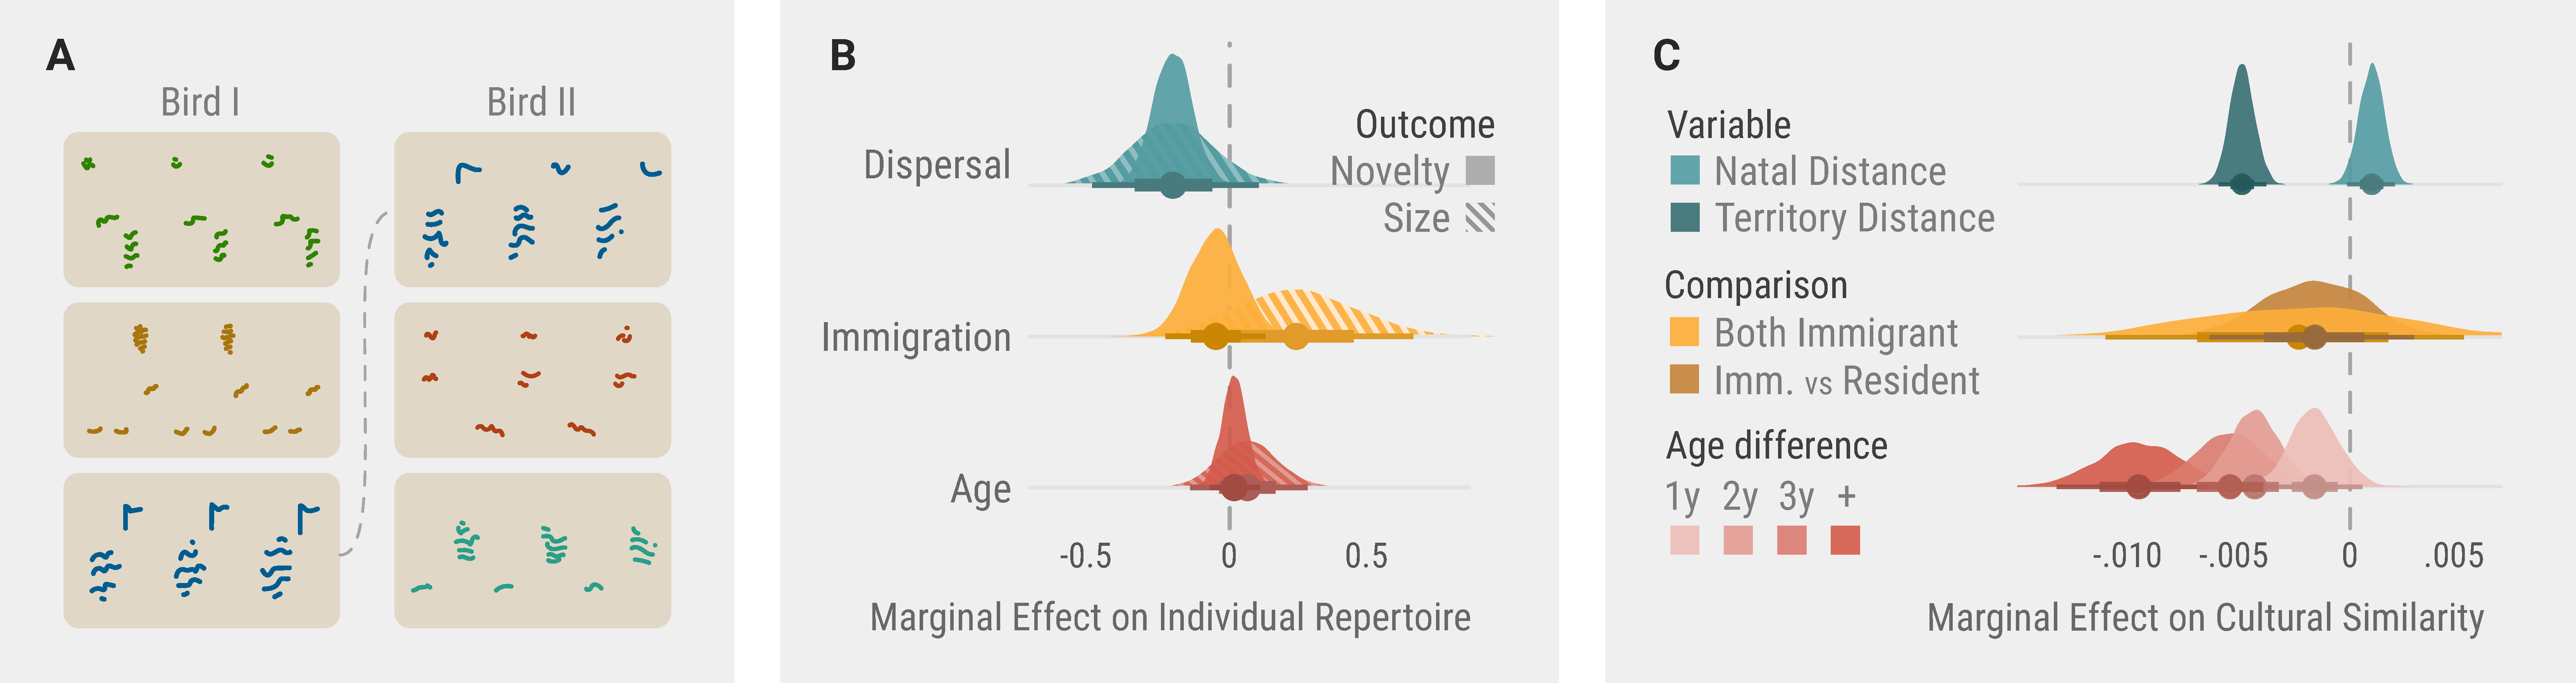
\includegraphics[width=\linewidth]{figures/chapter_4/FIG2.pdf}
    \mycaption{Individual and dyadic analysis of cultural diversity and similarity}{
        (A) Illustrative example showing the repertoires of two different birds in the population, with three songs in each, one of which is shared. Each sub-panel shows a cartoon spectrogram, with time in the horizontal axis and frequency in the vertical. Units not shown.
        (B) Marginal effects of dispersal, immigration status, and age on individual song repertoires, described in terms of their absolute size (the total number of distinct song types sung by that bird) and their uniqueness (how rare, on average, those songs are in the entire population within that year).
        (C) Marginal effects of dispersal, immigration status, and age on song repertoire similarity between individuals. Dispersal: Birds that are close neighbours are more culturally similar, regardless of where they were born, whereas natal distance may have a weak positive effect on cultural similarity. Immigration: There is no strong evidence that birds born outside the population are dissimilar from resident birds. Age difference: Birds are less culturally similar the greater the difference in their birth years, which evidences cultural change.
    }
    \label{c4_fig:individual}
\end{figure*}

Building on our understanding of cultural dynamics in relation to dispersal we expect that, when song learning is relatively precise and dispersal is limited, cultural differences between populations will accumulate, and immigration will introduce cultural novelty to the recipient population. However, the extent to which immigration introduces new cultural variants also hinges on an interplay between the species' learning programme, the timing of dispersal, and the spatial movements of individuals. Animals that learn first and then disperse, for example, may bring cultural novelty with them. But this is not the case for great tits, whose young disperse in late summer and autumn, shortly after achieving independence, learn their songs until the end of their first winter \autocite{rivera-gutierrez2011}, and become chiefly sedentary as adults \autocite{greenwood1979, dhondt1979, dingemanse2003}. In this species, then, we anticipate that immigrant birds will learn or retain songs they encounter upon arrival, either before or during the establishment of their territories \autocite{keen2020, graham2018}.

Indeed, in our population, we find no evidence that the repertoires of birds originating from outside the population significantly differ acoustically from those of resident birds ($mem = -0.002,~CI_{95\%}~[-0.006, 0.002]$; \figref[c]{c4_fig:individual}). This, in conjunction with the observation that song repertoire similarity between individuals is predicted by the distance between breeding territories ($mem = -0.005,~CI_{95\%}~[-0.006, -0.004]$; \figref[c]{c4_fig:individual}; \autoref{table:model_estimates}), supports the hypothesis that great tits are predominantly critical period learners that learn primarily from territorial neighbours after dispersal \autocite{mcgregor1982b, rivera-gutierrez2011}.

This leads to a somewhat contradictory scenario, however: immigrant birds, while not acoustically distinct, tend to have larger repertoires compared to their resident counterparts (\figref[b]{c4_fig:individual}; $P(\beta_{\overline{imm}.} > 0 | D) = 0.87,~mem=0.24,~CI_{95\%}~[-0.098, 0.593]$; \autoref{table:model_estimates}). At the group level, this small and uncertain effect amplifies, such that neighbourhoods with a higher proportion of immigrant birds do not have increased cultural diversity relative to the total number of songs ($mem=~0.002~CI_{95\%}~[-0.004, 0.007]$; \figref[a]{c4_fig:diversity}); but they do have a higher absolute cultural diversity---above what would be expected based solely on the number of birds ($P(\beta_{\overline{imm}.} > 0 | D) = 0.98,~mem=0.47,~CI_{95\%}~[0.1, 0.84]$; \autoref{fig:supp_absolute_cultural_diversity}, \autoref{table:model_estimates}). 

Previous research \autocite{verhulst1997}  has revealed that most birds arriving from outside the population disperse over two kilometres, significantly farther than the typical distances observed within the population (median for males = 558 metres \autocite{greenwood1979}). This extended dispersal may have qualitative consequences for cultural diversity, through a combination of factors: first, an initial exposure to songs from the source population; then, a heightened pressure to adopt vocalisations similar to those of territorial neighbours to avoid any social or reproductive costs associated with non-local signals, as seen in other species \autocite{payne1983, baker1981, mortega2014, lachlan2014, beecher2008}.

Finally, we find that individual turnover does not significantly affect cultural diversity or uniqueness, and we uncover an association between age structure and cultural diversity and uniqueness. Individuals of the same generation share the most similar song repertoires, and while age itself does not directly relate to changes in the repertoires of individual birds (\figref[b]{c4_fig:individual}), the acoustic similarity between pairs of individuals decreases as the age gap between them widens (\figref[c]{c4_fig:individual}; \autoref{table:model_estimates}). This is expected in birds that cease to learn new songs as they age, and has detectable consequences for neighbourhoods: those with a higher proportion of older individuals have heightened levels of cultural diversity and uniqueness (\figref[a\&c]{c4_fig:diversity}, \autoref{fig:supp_absolute_cultural_diversity}). Conversely, in areas where the majority of the population comprises younger birds surrounded by similar-aged peers, birds tend to produce fewer different song types that are also more common within the population (\textit{diversity:} $P(\beta_{\overline{age}} < 0 | D) = 1,~mem=0.021,~CI_{95\%}~[0.014, 0.027]$; \textit{uniqueness:} $P(\beta_{\overline{age}} < 0 | D) = 0.99,~mem=0.012,~CI_{95\%}~[0.005, 0.019]$; \figref[a\&c]{c4_fig:diversity}, \autoref{table:model_estimates}).

\begin{figure*}[!htb]
    \centering
    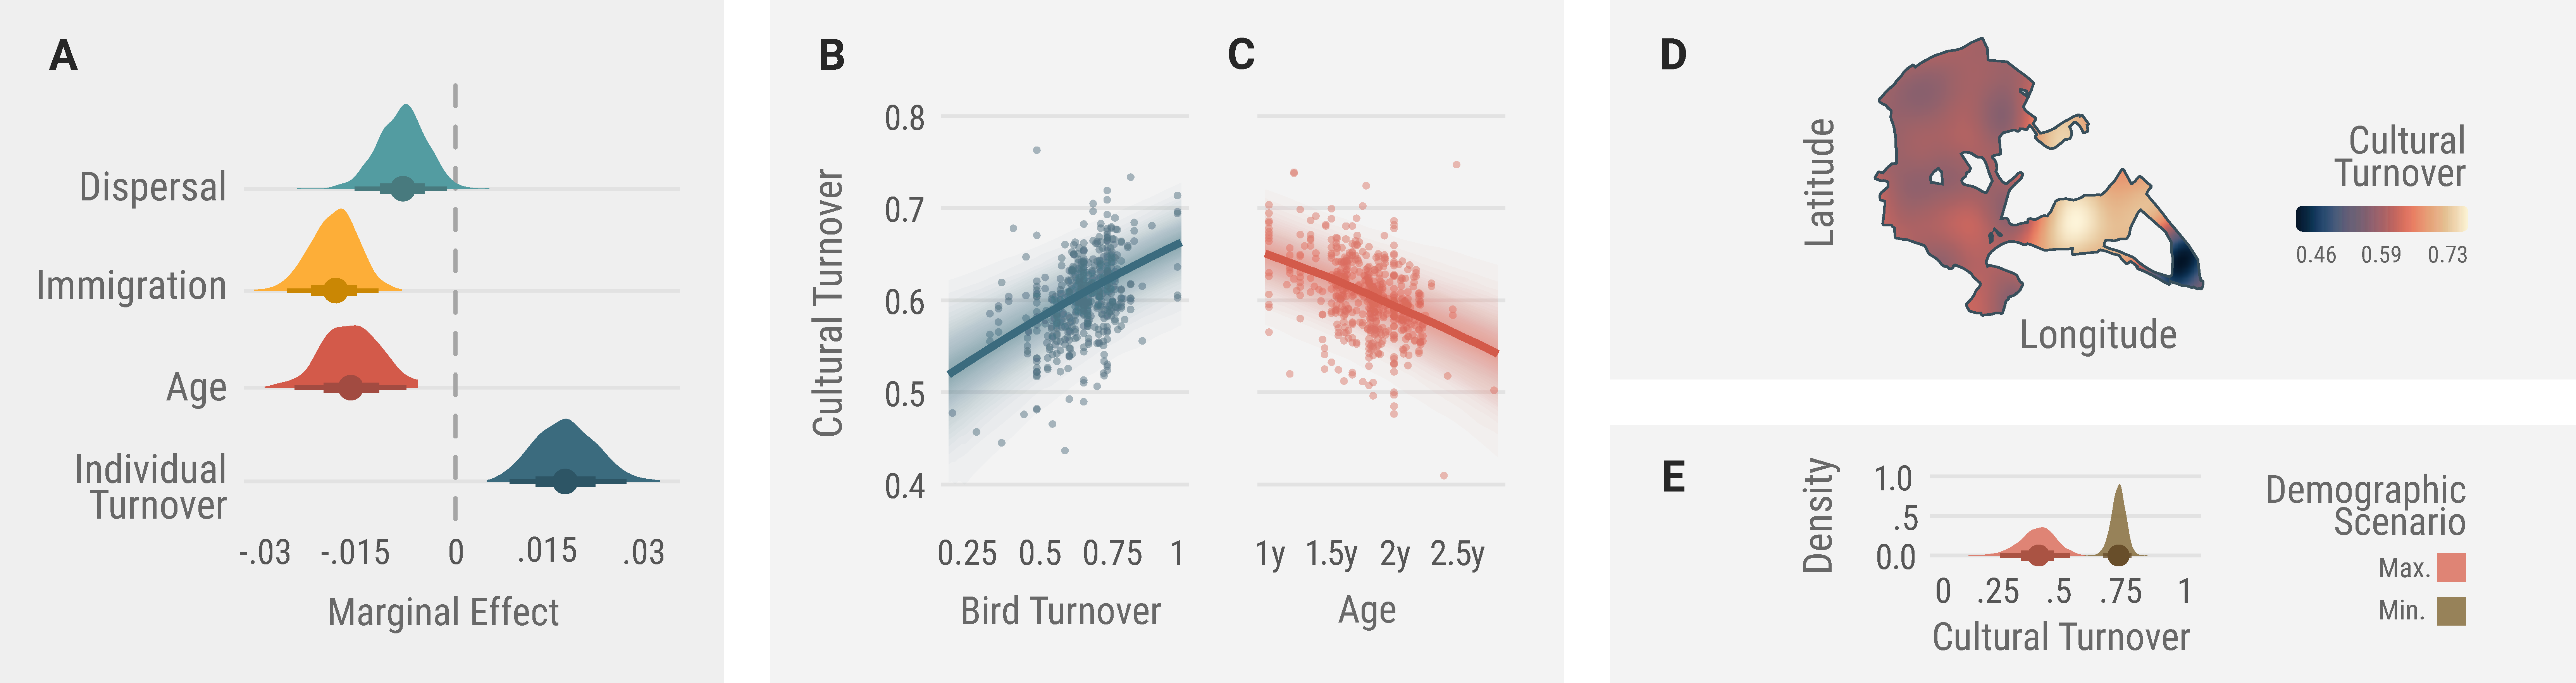
\includegraphics[width=\linewidth]{figures/chapter_4/FIG4.pdf}
    \mycaption{Influence of demographic variables on cultural turnover within neighbourhoods}{
        (A) Marginal effect at the means for mean dispersal distance, proportion of immigrant birds, average age, and individual turnover on the rate of cultural turnover within neighbourhoods
        (B and C) Adjusted predictions and partial residuals of the effects of the proportion of individual turnover on cultural turnover (B) and the effect of mean neighbourhood age on cultural turnover within neighbourhoods (C).
        (D) The population's average distribution of cultural turnover across space during the study period (2020-2022).
        (E) Posterior counterfactual predictions for two scenarios: all variables at their maximum (Max.) and minimum (Min.) observed values in the population, holding turnover constant at its mean value. Cultural turnover is expected to be over two times higher if neighbourhood dispersal, immigration and age are low, as they slow down cultural change.
    }
    \label{c4_fig:turnover}
\end{figure*}


\subsection{Demographic processes moderate the rate of cultural change at small spatio-temporal scales}

We now shift our focus from static measures of cultural diversity to cultural turnover, examining how quickly song types disappear from neighbourhoods and the consequences this has for their cultural makeup. The primary driver of cultural turnover within neighbourhoods is individual turnover (total effect $mem = 0.072$ $CI_{95\%}$ $[0.051, 0.093]$): as birds leave or die, many song types disappear with them, and the young birds that replace them might speed up the adoption of new song types \autocite{dyble2024}. Across the three-year study period, now considering the entire population, cultural turnover between consecutive years averages 0.45 (0.47 and 0.44; note that specific values are contingent on the granularity of song type definitions, see \hyperref[sc:manual-categorization]{manual categorization}). If all variants faced an equal chance of disappearing, this would quickly lead to complete cultural replacement. However, after a two-year gap, turnover only slightly increases to 0.59 (compared to an expected ~0.7; estimating the variance around these figures would require longer-term data). We anticipate this rate to taper further over longer periods, as rare variants encounter greater stochasticity while common songs endure, likely placing a ceiling on the long-term rate of cultural turnover (\figref[a]{fig:supp_song_frequencies}). Indeed, some common song types documented over four decades ago persist within the population \autocite{mcgregor1982b, keen2020}. This persistence might be due to different factors, like accurate learning based on song frequency, or strong tendencies to converge on certain song types \autocite{lachlan2018, tchernichovski2021, james2017, claidiere2007}.

After factoring in individual turnover, we examine how mean natal dispersal distance, the proportion of immigrant birds, and mean neighbourhood age affect cultural change within a neighbourhood. We find that higher levels of these factors correlate with slower cultural change  (\figref[a]{c4_fig:turnover}; \autoref{table:model_estimates}). Specifically, when individuals have dispersed over greater distances to get to their breeding neighbourhood, there is a high influx of immigrants, and the distribution of age is skewed towards older individuals, the model predicts slower cultural change, at less than half the rate compared to the converse scenario ($[0.66, 0.77]$$0.39$ $CI_{95\%}~[0.24, 0.51]$ vs. $0.72~CI_{95\%}$, as illustrated in \figref[e]{c4_fig:turnover}). This twofold difference in cultural turnover, based on realistic parameter values, is likely to significantly influence the cultural composition of neighbourhoods over time if it persists, highlighting the importance of the demographic structure of populations in also moderating the pace of cultural change.

The observed slowdown in cultural change due to dispersal and immigration aligns with our findings that dispersal homogenizes song repertoires and that immigrants tend to adopt the existing population's variants rather than introducing new ones (see \figref[a]{c4_fig:diversity} and \figref[a]{c4_fig:individual}). At the same time, our estimate for the effect of neighbourhood age ($P(\beta_{\overline{age}} < 0 | D) = 1,$ $mem=-0.044,$ $CI_{95\%}~[-0.063, -0.026]$; \figref[c]{c4_fig:turnover}) aligns with modelling work suggesting that learning from older individuals should slow down cultural change \autocite{kirby2021}. Indeed, age may serve as a brake on change, as older birds continue to sing song types that are becoming less frequent in the population, an idea supported by the observation that individual birds' repertoires are least similar when there is a large age difference (\figref[c]{c4_fig:individual}). The differences between the older and younger birds' repertoires also increases cultural diversity and uniqueness within neighbourhoods that include many older birds, as discussed above, suggesting an important role of age structure in shaping both cultural diversity and turnover.

\subsection{Consequences for cultural structure, stability and diversity}

Cultural traits, learnt bird song in this case, are shaped by many factors: some external, such as those discussed here, others intrinsic to learning and culture, and yet others that arise from selective processes driven by preference and function. Even within the confines of a relatively small population---Wytham Woods spans a mere four kilometres---we have been able to recover associations between heterogeneity in the demographic composition of neighbourhoods and cultural outcomes using a large dataset of song repertoires, and show that these are most likely underlied by differences in individual learning and exposure to cultural variants. In particular, we find that dispersal within the population reduces cultural diversity and uniqueness. Birds that were born outside the population seem to adopt existing song types rather than introduce new ones, but tend to have larger repertoires and so increase the absolute diversity of neighbourhoods. Birds of the same age tend to share similar song types, while neighbourhoods comprising both older and younger birds are more likely to exhibit a broader array of song types. Additionally, such neighbourhoods are more likely to host a greater number of birds singing rare song types, perhaps because, as we also find, aged neighbourhoods have slower cultural turnover. The main driver of cultural turnover is individual turnover, and, at the same time, longer postnatal dispersal distances, a higher proportion of immigrant birds, and an older population slow it down. 

Our study examines how demographic processes affect cultural diversity and the rate of cultural change on small spatial and temporal scales. We demonstrate that these factors can significantly influence cultural dynamics, but their impact on longer-term cultural diversification and persistence remains an open question. This emphasizes the need for both empirical studies and modeling efforts on cultural change to account for the population's demographic characteristics and their inherent heterogeneity across time and space. These factors shape individuals' exposure to cultural variants and learning opportunities, thereby influencing emergent group-level cultural dynamics.

\section{Methods}
\label{sc:methods}

\subsection{Resource availability}

The complete Wytham great tit song dataset is available in \href{https://osf.io/n8ac9}{osf.io/n8ac9}, and documented \href{https://nilomr.github.io/great-tit-hits/}{here}. The main repository with code and data to reproduce the analysis and figures in this article can be found at \href{http://github.com/nilomr/birdsong-demography}{birdsong-demography}.

\subsection{Data collection}

\subsubsection{Study system and fieldwork}

Great tits are small, short-lived birds---average lifespan: 1.9 years---that sing acoustically simple yet highly diverse songs. Each male great tit has a repertoire of one to over 10 song types, also referred to as song types, which are repeated multiple times in short bursts separated by longer periods of silence. Although detailed studies on how individual great tits learn their songs are limited, existing evidence suggests several key points. First, it appears that great tits do not learn their song repertoires from their fathers \autocite{mcgregor1982b}. Instead, their song development is influenced by the songs they encounter during their early life until they establish a territory and breed for the first time. We do not currently know how precisely great tits learn songs, or how social interactions affect the process. This period of vocal learning results in a final crystallized repertoire that remains relatively stable afterward---a process known as critical period learning \autocite{rivera-gutierrez2011}. Additionally, while there is evidence that birds can continue to learn to recognize new songs later in life (that is, learning for  discrimination, as opposed to learning for production), this ability seems to be limited compared to their early learning experiences \autocite{mcgregor1986}. Furthermore, females are able to individually recognize males based on their songs \autocite{lind1996} and, even across a large population, individual song renditions can accurately indicate the identity of the bird producing them \autocite{merinorecalde2023a}.

During the breeding season, from March to June, great tit pairs are socially monogamous and defend territories around their nests \autocite{hinde1952}. In Wytham Woods, Oxfordshire, UK (51\degree46 N, 1\degree20 W), a population of these birds has been the focus of a long-term study since 1947 \autocite{lack1964}. Wytham Woods is a semi-natural, predominantly deciduous and partly discontinuous woodland that spans an area of approximately 385 hectares and is surrounded by farmland. Most great tits in this population breed in nest boxes with known locations, and the majority of individuals are marked with a unique British Trust for Ornithology (BTO) metal leg ring as either nestlings or adults. The birds were not provided with supplementary sources of food during the study.

We collected data from late March to mid-May during the 2020, 2021, and 2022 breeding seasons. Every year, fieldworkers checked each of the 1018 nest boxes at least once a week before and during the egg-laying period, which typically lasts from one to 14 days \autocite{Perrins1965}, and recorded the identities of breeding males and females, the dates of clutch initiation and egg hatching, clutch size, and fledgling number and condition under standardized protocols. We found the first egg date by assuming that one egg is laid every day and counting back from the day of observation. In cases where we did not observe the chicks on their day of hatching, the actual hatching date was determined by assessing the weight of the heaviest chicks and extrapolating their age from established growth curves \autocite{cresswell2003, gibb1950}.

Nest box occupancy and breeding density vary across the study area, with some areas having a higher density of nest boxes and a higher proportion of occupied boxes, which we account for in some of our analyses as described in the sections below. In the years of our study,  261, 289 and 278 nest boxes were occupied by pairs of great tits, with 173, 184 and 184 that led to successful breeding attempts where at least one chick fledged. See \autoref{fig:supp_study_site} for a map of the study site and sampling locations.

To record the vocalisations of male great tits we took advantage of their behaviour during the reproductive period, when they engage in continuous singing near their nests at dawn before and during egg laying \autocite{mace1987}. Collectively, this vocal display is referred to as the dawn chorus, and has been demonstrated to yield a reliable estimation of the song repertoire of individuals when recorded in full \autocite{rivera-gutierrez2012, vanduyse2005}. As soon as we suspected that a pair of great tits were using a nest box---based on nest lining materials, egg size if present, or other signs of activity---we deployed an autonomous sound recorder nearby. The microphone faced upwards and slightly away from the nest box, aligning with the nest box entrance hole's direction. The birds sang near the recorder: although we did not gather data on this aspect, our anecdotal observations were in line with a different population where the average distance to the nest box while singing was 10 metres \autocite{halfwerk2012}. 

This approach is supported by previous studies on great tit dawn song \autocite{keen2020, naguib2019,snijders2015, boucaud2016, boucaud2016a}, as well as our observations that: (a) recordings from consecutive days contain renditions of the same song types clearly sung by a single individual cycling through its repertoire, (b) renditions of the same song types across different days can be assigned to a single individual by our deep metric learning model (see \hyperref[sc:song-similarity]{deep metric learning model training}), and (c) when we recapture the same bird in a different field season (often in the same location due to adult site fidelity), we can easily match its songs to those previously recorded. To further ensure that we were recording the correct birds, we discarded rare recordings with more than one vocalizing bird unless one was distinctly louder than the others during the segmentation process. Additionally, we excluded all songs with a maximum amplitude below $-16$ dB, calculated as $20\log_{10}\left(\frac{A}{A_0}\right)$, with $A=5000$ and $A_0=32767$ (the maximum value for 16-bit digital audio). This threshold was established based on observations showing that an amplitude cutoff greater than 4000 unambiguously differentiated the focal bird from its closest neighbours when simultaneous recordings from nearby spatial locations captured multiple birds. It is important to note that these values are not calibrated and are relative to our recording equipment and settings, as well as other factors like sound directionality and vegetation cover.

Our recording efforts captured birds belonging to around half of all breeding attempts \autoref{fig:supp_neighbourhood_sampling} (including both successful and unsuccessful attempts, with or without linked individual data), which may result in some rare song types being underrepresented or undetected if they are sung by less successful or late-breeding individuals. We do not currently have evidence suggesting this skews our results, but it remains a plausible consideration. Importantly, the birds that we did record are representative of the neighbourhood's breeding density, dispersal distances, contribution of immigration, and age distribution (see  \autoref{fig:supp_neighbourhood_sampling}). In a related way, those birds that sing more frequently are more likely to be recorded , but as these are also likely to be the primary contributors to the local song pool, we believe our sample adequately reflects the overall song repertoire of the breeding population in each area.

Our recording efforts captured song repertoires from birds belonging to approximately half of all breeding attempts \autoref{fig:supp_neighbourhood_sampling}, including both successful and unsuccessful attempts, as well as individuals with and without linked data. This song sampling density, while high for this kind of field study, could theoretically result in some rare song types being undersampled---particularly if rare song types are primarily sung by unsuccessful or late-breeding individuals---but we have no evidence suggesting that this is the case. A related potential issue is that birds that sing more frequently might be more likely to be recorded, but as these individuals are also the primary contributors to the local song pool due to their higher song output we are confident that our data provides a representative sample of the song repertoire of the breeding population in each area. Importantly, the birds that we recorded are representative of the neighbourhood's composition in terms of breeding density, dispersal distances, contribution of immigration, and age distribution (see  \autoref{fig:supp_neighbourhood_sampling}).
 
For this study, we calculated postnatal dispersal distance was as the straight line distance from the natal site to the breeding site. The dispersal distances of birds classed as immigrants (not ringed as chicks in the population) are not known, but most are thought to come from other populations at least 1 km, and likely more than 2.5 km, away \autocite{verhulst1997, quinn2011}. We determined age based on the year of hatching for birds born in the population and using plumage characteristics for immigrants, which are most often caught as yearlings (76\%)---allowing us to age them accurately \autocite{woodman2023}.

All work involving birds was subject to review by the University of Oxford, Department of Zoology, Animal Welfare and Ethical Review Board (approval number: APA/1/5/ZOO/NASPA/ Sheldon/TitBreedingEcology). Data collection adhered to local guidelines for the use of animals in research and all birds were caught, tagged, and ringed by BTO licence holders (NMR's licence: C/6904).

\subsubsection{Recording equipment and schedule}
We used 60 (30 in 2020) AudioMoth recorders \autocite{hill2019}, which were housed in custom-built waterproof enclosures. Recording began approximately one hour before sunrise (05:36 -- 04:00 UTC during the recording period) and consisted of seven consecutive 60-minute-long recordings with a sample rate of 48 kHz and a depth of 16-bit. To sample as many birds as possible, we left each recorder at the same location for at least three consecutive days before moving it to a different nest box. We relocated 20 recorders (10 in 2020) every day throughout the recording period.

\subsection{Data processing and annotation}

We processed and annotated the song recordings, 109,963 in total, from 299 repertoires belonging to 242 known birds, using custom software and scripts written in Python 3 \autocite{vanrossum1995} and the open source package \texttt{pykanto} \autocite{merinorecalde2023}. These are available from \href{https://github.com/nilomr/great-tit-hits-setup}{github.com/nilomr/great-tit-hits-setup} \autocite{nilo_gretidataset_setup_2023}. Our annotated dataset and a detailed description of the process can be found in Merino Recalde et al \autocite{merinorecalde2023a}. Below we provide a narrative summary of the subsequent characterisation of song similarity and song types.

\subsection{Characterizing repertoire similarity}

Our analyses require i) a measure of the acoustic similarity between any two birds for the individual-level analyses, and ii) a way to identify categorical song types for the neighbourhood analyses. The underlying assumption is that song repertoires will be more similar if one bird has learned it at least in part from a second, or if they have both learnt from other individuals who are themselves similar due to intergenerational cultural descent. There is no single optimal solution for this problem, both due to technical challenges and because we do not know enough about song perception and learning mechanisms in this species. There are three main possible approaches, each with its own advantages and disadvantages, which we describe below.

\phantomsection
\subsubsection{Continuous similarity (individual-level analyses)}
\label{sc:song-similarity}

Traditional methods used to compare bird vocalisations include visual inspection of spectrograms and measurement of hand-picked acoustic features. However, these approaches have limitations in dealing with noise and variations in performance, and can be extremely time-consuming. So, instead, we adopted a data-driven approach by training a Vision Transformer (ViT) model for feature extraction in a metric learning task on spectrogram representations of great tit songs. Our goal was to create a similarity space based on inherent variation in the data, using categorical labels of song types sung by individual birds, which we know to be perceptually and behaviourally significant \autocite{lind1996}. Further details, data, and code to reproduce this process are available at \autocite{merinorecalde2023} and \autocite{merinorecalde2023a}; we include a summary here.

We optimized model performance using Triplet loss, a loss function that ensures the projection of a positive sample (belonging to the same class as the anchor point) is closer to the anchor's projection than that of a negative sample (belonging to a different class) by a specified margin \autocite{hermans2017, hoffer2018}. During training, we mined hard triplets---where the negative sample is closer to the anchor than the positive---and used the Adam optimizer with a fixed learning rate of $1 \times 10^{-5}$.

To prevent the model from overfitting to irrelevant features within localized portions of the training data or learning background noise, we applied various train-time data augmentation techniques \autocite{mumuni2022,perez2017,shorten2019}. These included random cropping in the time domain, dropping out parts of the spectrogram, adding Gaussian and multiplicative noise, equalization, sharpening, changes to brightness and contrast, blurring, and slight shifting in both time and frequency domains. This leads to a more robust model that can generalize better and is not influenced by differences in background noise.

Finally, we used the resulting model to calculate feature vectors for each song in the dataset (109,963 samples x 384 dimensions), which serve as compressed representations that can be used to compare them. Great tits have variable repertoire sizes and there is no evidence that they ever learn them en bloc \autocite{mcgregor1982b, rivera-gutierrez2010a}. Therefore, the simplest continuous measure (an average pairwise Euclidean distance between all songs) would mask any signatures of learning if the average repertoire similarity is similar across the population, and does not take into account the asymmetry in total repertoire size. To improve on this, we define repertoire similarity as the average minimum Euclidean distance (\text{AMED}), given by

\begin{equation} 
\label{eq1}
\text{AMED} = \frac{1}{|A|} \sum_{a \in A} \min_{b \in B} \left| a - b \right|_2
\end{equation}

where we compare each song feature vector $a$ in set $A$ with all song feature vectors $b$ in set $B$ and compute their Euclidean distance $\left| a - b \right|_2$. We then retain the minimum distance for each element in set $A$ and obtain the \text{AMED} by averaging these minimum distances over all elements in set $A$.
The main advantage of this approach is that it allows us to avoid imposing discrete population-wide song categories. On the other hand, if song learning is categorical and not very precise in terms of fine song structure, this method could underestimate it or fail to detect it. We used this approach for all individual-level analyses in this paper. 

\subsubsection{Automated clustering (first step for neighbourhood analyses)}

Instead of calculating a continuous measure of repertoire similarity, we can build a pairwise distance matrix for all songs, assign them to discrete clusters using a clustering algorithm, and then calculate the intersection between repertoires by using the Jaccard coefficient or modelling it as a binomial process, with $n = $ the combined repertoire size and $s = $ the number of songs in the same cluster. Here we used UPGMA hierarchical clustering and dynamic tree-cut techniques to classify the syllables into distinct types (since songs consist of repeated syllables, syllable and song types are synonymous in this species). We allowed a minimum cluster size of 1 to ensure the representation of rare song types. The usefulness of this method relies on the global properties of the embedding space derived from the \hyperref[sc:song-similarity]{continuous similarity} process. In a low-dimensional space where linear distances effectively capture meaningful variation, creating clusters by cutting the hierarchical tree at different heights yields varying cluster counts while maintaining meaningful groupings. However, in a high-dimensional space where global distances are not meaningful, only relatively small clusters of nearby points remain interpretable. This is the case with our dataset and embedding space: we find that the method reliably groups song renditions by the same bird across different years, alone or together with other birds with highly similar songs, yet consistently splits songs that are similar by human (and perhaps great tit \autocite{falls1982}) standards, ultimately leading to a very large number of clusters (the most stable clustering solutions were close to the total number of different individual song types, >1000). Due to these issues, we did not directly use song types defined in this way, and performed an additional manual categorization step.

\phantomsection
\subsubsection{Manual categorization (second step for neighbourhood analyses)}
\label{sc:manual-categorization}

Our neighbourhood-level analyses require that we define discrete cultural units (namely, population-wide song types). With over 100,000 songs, our dataset is much larger than is common in the field and would have been impossible to label entirely manually. Instead, we used the output of the automated clustering process described above, consisting of labelled song repertoires (birdID x song type). This made the problem 57 times smaller: 1920 song types that were already assigned to small clusters of highly similar songs, which we reviewed manually using the criteria followed by McGregor and Krebs \autocite{mcgregor1982b, mcgregor1982, mcgregor1981} and subsequent work \autocite{baker1987, falls1982, fayet2014, hutfluss2022}.
This process is both inevitable and partly subjective. However, despite its clear problems, human perceptual judgments might be our best available substitute for those of the birds for some tasks (but see recent work by Morfi et al. \autocite{morfi2021} and  Zandberg et al. \autocite{zandberg2022}). Indeed, across fields, advanced classification algorithms are routinely evaluated against ground truth created by humans, and this is also the case in bird song research.

Following common practice in the field, we statistically validated our resulting 335 manually assigned labels to evaluate whether if they represent quantitatively robust clusters. To do this, we retrained the ResNet50-based classifier described in Merino Recalde \autocite{merinorecalde2023} on a random subset of labelled song spectrograms data and obtained an accuracy of 0.87 on the validation set (see other metrics in the repository). For comparison, an equivalent process by Fayet et al. \autocite{fayet2014} was able to reach 0.71 accuracy for 374 songs. We further explored the result by building a dendrogram based on the confusion matrix during test time and reviewing classes that were not well supported, which, following  \autocite{fayet2014}, led us to collapse seven classes into two. With the caveats already mentioned, this means that our classification following McGregor and Krebs \autocite{mcgregor1982b} is indeed successful at finding song type clusters that reduce intraclass variation.

Most of the great tits in our population sing some variation of the well-known 'tea-cher, tea-cher' song, These are harder to assign to discrete classes than rarer songs with more complex structures, a problem that is not restricted to our dataset: regions of the acoustic space with more data are harder to cluster because they often contain more variation and overlap, making it difficult for algorithms (or humans) to find clear boundaries. In contrast, fewer, distinct songs make clustering simpler. As mentioned in the main body of the article, the consequence of this for any analysis is that the absolute estimates of cultural turnover depend on the granularity of this clustering process. Were we to lump most 'tea-cher' songs together, as McGregor and Krebs \autocite{mcgregor1982b} do, the estimates of turnover would become lower---but, crucially, any relative differences across time or space remain the same. Indeed, precisely quantifying turnover using categorical metrics might be altogether impossible in some species, because song categories are not likely to be natural kinds be    yond the scale of interacting neighbours. 

See \autoref{fig:supp_song_typle_clusters} for examples of song types defined in this study. The exact code used to perform this song type validation process, along with the figures generated during it, can be found in \href{https://github.com/nilomr/wytham-songtype-validation/blob/main/notebooks/4_train-model.ipynb}{the main narrative notebook} and \href{https://github.com/nilomr/wytham-songtype-validation}{a dedicated repository}.

\subsection{Re-identifying individuals from their songs}

In some cases, we failed to capture or identify birds using PIT (Passive Integrated Transponder) tags, as tags sometimes malfunction, birds can be difficult to catch, or disappear before their chicks are old enough to attempt this.  We were able to match an additional 31 song repertoires belonging to this subset of birds with existing individual IDs by using the deep metric learning model (ViT) described earlier to recognize individual songs. This increased the number of identified repertoires from 299 to 330, belonging to the same 242 unique birds. We summarise the process here, but see also \autocite{merinorecalde2023a} for details on model design and training.

Briefly, we calculated pairwise song distances using the feature vectors obtained from a vision transformer on a metric learning task. This model achieved a mean average precision at 5 (mAP\@5) of 0.98 and a cumulative matching characteristic at 1 (CMC\@1) of 0.98, which roughly means that in 98\% of the queries made to the similarity space on a held-out test dataset of known songs the returned candidate song type by a bird is the correct one. Given that the model was trained on almost 2000 classes, this means that there is enough individual information contained in each song type to distinguish between birds with very high confidence: even when birds sing very similar songs, this model can still tell them apart.

We then use these distances between song embeddings to infer when two repertoires belong to the same bird, even if had not been physically identified more than once. To do this, we set very conservative criteria: that a minimum of two songs are more similar than the 0.025 quantile of the distribution of distances for all song types sung by birds already known to be different, or 0.9, and that the bird is no more than 100 metres apart from the reference bird. If we query the metric learning model across the songs of the entire population, which increases the chances of a false positive, we find that the percentage of wrongly assigned birds in our ground truth data (birds that we have physically re-identified across years) is 0.3\%, or 34 out of 11,359 unique comparisons if we only use acoustic distance---further reduced to 0.04\%, or 4 out of 11359, if we also add the spatial constraint (see \autoref{fig:supp_acoustic_distance_threshold} for a graphic explanation).

\subsection{Quantification and statistical analysis}

\subsubsection{Modelling pairwise similarity and individual repertoires}

It is common for analysis of song similarity to fit simple linear regression models using all pairwise comparisons in a population. However, this leads to very strong pseudo-replication and, therefore, an increased chance of Type I errors. To avoid this, we treat our song similarity data as a fully connected network and build Bayesian multilevel models with a multi-membership structure and the pairwise $\text{AMED}$ described above as the response variable. The full model specifications can be found in the \href{https://github.com/nilomr/birdsong-demography}{main repository} for this project; also see a summary in \autoref{table:model_info} and variable descriptions in \autoref{table:variable_key}.

\paragraph{Individual repertoires}
We first modelled individual repertoire size using Poisson and negative binomial models, but this led to poor performance as assessed through posterior predictive checks (both underestimation of mean values and either under or over-estimation of very low repertoire sizes). Instead, we built continuation ratio models, a type of sequential ordinal model where reaching a particular level (number of song types in the repertoire) requires first reaching all lower levels \autocite{chambers2023, warti2020}. $rep_{m_1}$, $rep_{m_{1.1}}$, and $rep_{m_{1.2}}$ estimate the association between immigrant status, distance dispersed, age, and repertoire size. Three further log-normal models, $repnov_{m_1}$, $repnov_{m_{1.1}}$, $repnov_{m_{1.2}}$, do the same for the average cultural uniqueness of individual repertoires, defined as one minus the mean of the relative frequencies of each song type present in the repertoire.

\paragraph{Pairwise similarity}
Our first model ($disp_{m_1}$) explores the interaction between natal distance, that is, the distance between the nests where two resident birds were born, and the distance between the centre of their breeding territories, adjusting for year and absolute age difference. We do not have direct information on how long birds have spent around one another, so instead we estimate the effect of the interaction of the distance at which they were born and the distance at which they subsequently breed: If both are small, they will have had more opportunities for interaction and learning. We extract predictions for the interaction and calculate marginal effects at minimum distances, to answer the questions 'How does cultural similarity change with distance for birds that were born nearby' and 'Does how close a bird was born matter for birds that hold territories nearby'. We use a similar model structure ($age_{m_1}$) to estimate the marginal effects of the absolute age difference, this time adjusting for the natal and territorial distance between birds. Then, to study the effect of immigration, we fit a model ($imm_{m_1}$) with the possible combinations of immigration status (both immigrant, both residents, one of each) and adjust for age difference and territorial distance. 

\phantomsection
\subsubsection{\nmu Modelling group-level outcomes}
\label{sc:group-properties}


\paragraph{Defining neighbourhoods and their demographic properties}

Song turnover, diversity, and uniqueness are group-level properties. However, our study lacks naturally occurring distinct subpopulations that we can use as units for analysis. Rather than partitioning the population using a discrete polygonal grid or non-overlapping areas, we opted to model neighbourhoods continuously across space, defining a radius of 200 m around each of 549 nest boxes that were occupied at least once during the study \autocite{fayet2014}, which we then sampled across the duration of the study. This radius is necessarily arbitrary but strikes a good compromise between capturing the relevant spatial scale at which vocal interactions occur, which extends up to around 180 metres \autocite{bircher2021, blumenrath2004}, and maintaining an adequate sample size in areas of low density (neighbourhood sizes range from $7$ to $60$, mean $30.3\pm14.9$). Importanty, neighbourhoods defined in this way are highly non-independent, so we model both this methodological spatial dependence and other sources of complex spatial autocorrelation intrinsic to the study site by including a 2D Gaussian process (GP), which estimates a length-scale parameter defining a variance-covariance matrix for the spatial locations based on their distance \autocite{dearmon2016, gelfand2016, wright2021}. We confirmed that this eliminated the residual spatial autocorrelation via Moran's I tests. Note that we fit a separate GP for each year, as treating the spatial dependence as fixed across the study duration, as is often done, risks further underestimating uncertainty.

\noindent
We define our predictor variables in the following way: 
\begin{itemize}
    \item Individual turnover is the proportion of birds that were not already in a neighbourhood in the preceding year.
    \item Dispersal is the mean of the distances, in metres, that birds in the neighbourhood travelled to get from their natal territories to their current territories if they were hatched within the Wytham population. 
    \item Immigration is the proportion of birds that were not ringed as nestlings in the population, and 
    \item Neighbourhood age is the mean age of the birds within it. 
\end{itemize}

\noindent\autoref{fig:supp_neighbourhood_sampling} illustrates that our sampling process did not introduce bias into any of these predictor variables: the birds from which we recorded song repertoires were, on average, representative of the true neighbourhood composition. \autoref{fig:supp_demo_variables} shows the distribution of the 'raw' variables across the study site.

\paragraph{Operational definitions of cultural diversity, uniqueness, and turnover}
\label{sc:op-definitions}

In this paper we use simple descriptions of cultural diversity, cultural uniqueness, and cultural turnover that intuitively capture relevant aspects of the collective song repertoires of neighbourhoods in relation to the rest of the population. We define our outcome variables in the following way:

\begin{itemize}
    \item Relative cultural diversity ('diversity'): the ratio of distinct song types recorded in a neighbourhood to the total number of songs recorded in that neighbourhood. Higher values indicate that there are more distinct song types in the neighbourhood relative to the total song output.
    \item Absolute cultural diversity: the number of distinct song types recorded in a neighbourhood. Higher values indicate that there are more distinct song types in the neighbourhood.
    \item Uniqueness index: the complement of the logarithm of the mean population-wide frequency of the song types present in a neighbourhood. Higher values indicate that the songs in the neighbourhood are on average less common in the population.
    \item Cultural turnover: the proportion of distinct song types recorded in a neighbourhood that were not present in the previous year. Higher values indicate that the neighbourhood's song repertoire has changed more from one year to the next.
\end{itemize}

In this way, 'diversity' describes the relative proportion of distinct songs in a neighbourhood, and 'uniqueness' refers to how uncommon, on average, the songs of the birds in a neighbourhood are. These two ways of characterizing cultural diversity are (as expected) anti-correlated in our study site due to the effect of sampling: more frequent songs are sampled more readily, causing larger sample sizes---neighbourhoods with more density and therefore songs---to yield lower average estimates of diversity and higher average estimates of uniqueness, in a nonlinear manner. Once this is adjusted for, which we do by including  a GAM term capturing the nonlinear effect of the sample size, diversity and uniqueness are positively correlated, as expected (see \autoref{fig:supp_song_sampling}; models $nov_{m_2}$ and $nov_{m_{2.1}}$; spatial distribution of these variables in \autoref{fig:supp_cultural_variables}). All the relevant models adjust for these effects of neighbourhood density and sampling.

\paragraph{Models}

To study the effect of dispersal and immigration on local cultural diversity and uniqueness, we built log-normal models ($div_{m_1}$, $nov_{m_1}$) and estimated the marginal effects of the proportion of immigrants, mean dispersal distance, and mean neighbourhood age, while also adjusting for individual turnover, year, and spatial dependence. Lastly, to examine whether the effects of immigration and dispersal on cultural diversity were related to individual differences in repertoire size and uniqueness, we fit two further models predicting the absolute number of distinct song types in a neighbourhood while also adjusting for the number of birds ($div_{m_2}$) and the number of songs ($div_{m_{2.1}}$).

The rate of song cultural turnover was the response variable in two models: one ($turn_{m_1}$) trying to estimate the total effect of turnover and a second ($turn_{m_2}$) estimating the marginal effects of the proportion of immigrants, mean dispersal distance, and mean age while also adjusting for individual turnover, year, and spatial dependence. In both cases, we modelled the response distribution as a truncated log-normal with a hurdle (logistic) part to account for the zeroes. 

\subsubsection{Model estimates and reporting}

We built the models and approximated the posterior distributions of the parameters of interest using brms \autocite{brms2017}, an interface to the Hamiltonian Monte Carlo engine Stan \autocite{stan2023}. We then processed the posterior distributions with the help of the marginaleffects package \autocite{marginaleffects}. We checked model convergence via the effective number of samples, visual inspection of the chain trace plots, and the Gelman-Rubin diagnostic. Estimation in a Bayesian framework returns a posterior distribution of possible values instead of point estimates. By convention, we report posterior central estimates (means or medians) and their 95\% credible intervals, but also include plots with full posteriors. Note that categorical predictors are dummy-coded and continuous predictions z-score transformed.

For each parameter of interest, we calculated predictions or marginal effects at the means or other relevant values.  Regression plots show predicted values of the mean and their credible intervals, as well as partial residuals adjusted to the means or other relevant values of the explanatory terms included in the model \autocite{fox2018, larsen1972}. We have tried to build reasonable models, but even then our estimates should not be interpreted causally. \autoref{fig:supp_pp_checks} shows posterior predictive checks for all models in the study. See the software section at the end for a complete list of libraries used in the various analyses and the code repository for full model specifications.

\subsubsection{Software}
\begin{sloppypar}
Song processing and analyses were carried out using pykanto \autocite{merinorecalde2023} and rely on the following open-source scientific libraries or tools: numpy \autocite{numpy2020}, scipy \autocite{scipy2020}, pandas \autocite{pandas2023}, numba \autocite{lam2015}, pytorch \autocite{pytorch2019}, torchvision \autocite{torchvision2016}, pytorch lightning \autocite{pytorchlightning2019}, tqdm \autocite{tqdm2019}, ray \autocite{moritz2018}, soundfile \autocite{bechtold2022}, umap \autocite{mcinnes2018},  joblib \autocite{joblib2020}, hdbscan \autocite{mcinnes2017}, seaborn \autocite{Waskom2021}, scikit-image \autocite{scikitimage2014}, librosa \autocite{mcfee2015}, bokeh \autocite{bokeh2018}, ujson \autocite{ujason2023}, psutil \autocite{psutil2023}, attrs \autocite{schlawack2019}. We also used R version 4.2.1 \autocite{base} and the following R packages: bayesplot \autocite{bayesplot2019, bayesplot2022}, box \autocite{box}, brms \autocite{brms2017, brms2021}, ClustGeo \autocite{ClustGeo}, colorspace \autocite{colorspace2020a}, config \autocite{config}, devtools \autocite{devtools}, DHARMa \autocite{DHARMa}, fs \autocite{fs}, ggdist \autocite{ggdist}, ggraph \autocite{ggraph}, httpgd \autocite{httpgd}, igraph \autocite{igraph2006, igraph2024}, insight \autocite{insight}, kableExtra \autocite{kableExtra}, languageserver \autocite{languageserver}, marginaleffects \autocite{marginaleffects}, modelsummary \autocite{modelsummary}, patchwork \autocite{patchwork}, progress \autocite{progress}, renv \autocite{renv}, rprojroot \autocite{rprojroot}, scales \autocite{scales}, scico \autocite{scico}, sf \autocite{sf2018, sf2023}, svglite \autocite{svglite}, terra \autocite{terra}, tidygraph \autocite{tidygraph}, tidyverse \autocite{tidyverse}, viridis \autocite{viridis}. See the code repositories for specific versions of these libraries.
\end{sloppypar}

\section{Acknowledgements}

We thank all those who have contributed to the long-term nest box study in Wytham Woods and the collection of associated data. We also thank three anonymous reviewers for their constructive feedback. This work was supported by a Clarendon-Mary Frances Wagley Graduate Scholarship and an EGI scholarship to Nilo Merino Recalde, and made use of the University of Oxford Advanced Research Computing facility \autocite{richards2015}.

\section{Author contributions}
\textbf{Nilo Merino Recalde}: Conceptualization, Methodology, Software, Formal analysis, Investigation, Data Curation, Writing - Original Draft, Writing - Review \& Editing, Visualization. 
\textbf{Andrea Estandía}: Investigation, Data Curation, Writing - Review \& Editing.
\textbf{Sara C. Keen}: Writing -- Review \& Editing.
\textbf{Ella F. Cole}: Supervision, Project Administration.
\textbf{Ben C. Sheldon}: Supervision, Project Administration, Writing -- Review \& Editing, Funding Acquisition.


\printbibliography

\onecolumn
\supplementarysection

\begin{longtblr}[
    theme=ntabs,
    caption = {Model variable key}, % Table caption
    label = {table:variable_key} % Label for cross-referencing
  ]{
    colspec = {X[l] X[6,l]}, % Define column specification
    column{1}={colsep=15pt},
    rowhead=1,
    row{odd} = {tablegrey}, % Shading for odd rows
    cells = {font = \fontsize{8pt}{8pt}\selectfont},
    row{1} = {tableheadgrey, font=\fontsize{8pt}{8pt}\selectfont\bfseries} % First row is bold
  }
  
  Variable & Description \\
  
  repertoire\_size & Number of distinct song types sung by an individual \\
  immigrant & Immigrant status (hatched in the population / not hatched in the population)  \\
  sampling\_effort & Total number of recordings obtained for this individual \\
  year & Year in which the repertoire was recorded \\
  father & ID of the male; BTO (British Trust for Ornithology) ring number \\
  dispersal\_distance & Postnatal dispersal distance, in metres, from the natal nest box to the breeding nest box \\
  age & The age of the bird. This is exact if the bird was ringed as a pullus in the population, or approximate (based on plumage moult) otherwise \\
  average\_frequency & The mean of the frequency of each song in a bird's repertoire in a given year \\
  mean\_dist1 & Average minimum Euclidean distance between the repertoires of two birds \\
  natal\_distance & Distance in metres at which two birds were born \\
  nest\_distance & Distance in metres at which two birds bred \\
  year\_born\_diff & The absolute difference between the birth years of two birds \\
  mm(...) & Multi-membership grouping term for the similarity network \\
  resident\_status & Origin of a pair of birds: both, one or neither were hatched in the population \\
  prop\_immigrant & Proportion of  the birds in a neighbourhood that were not hatched inside the population \\
  mean\_dispersal\_\allowbreak distance & Mean postnatal dispersal distance, in metres, of the birds in the neighbourhood\\
  prop\_same\_birds &  Proportion of the birds in a neighbourhood that were already there the year before \\
  mean\_age & Mean age of the birds in a neighbourhood \\
  diversity & The ratio of distinct song types recorded in a neighbourhood to the total number of songs recorded in that neighbourhood\\
  n\_current\_songs & Absolute number of songs in a neighbourhood, where each different song types is counted as many times as it appears. This variable correlates with neighbourhood size, and we use to more precisely adjust for the fact that some birds sing more song types \\
  gp(x, y) & 2D Gaussian process to model spatial dependency in the data  \\
  n\_unique\_\allowbreak current\_songs & Number of distinct song types within a neighbourhood in a year, counting each different song type only once\\
  uniqueness &  Quantified as one minus the logarithm of the mean population-wide frequency of the songs in the repertoire of either a bird or an entire neighbourhood within a given year  \\
  recorded & Number of birds recorded singing in a neighbourhood, which is linearly correlated with neighbourhood size \\
  prop\_shared & Proportion of the song types in a neighbourhood that were already present. Reported as 1- prop\_shared: 'song turnover'\\
  \end{longtblr}
\begin{longtblr}[
  theme=ntabs,
  caption = {Model information}, % Table caption
  label = {table:model_info} % Label for cross-referencing
  % note{a} = {Continued from previous page}, % Note for continued header
  % note{b} = {Continued on next page}, % Note for continued footer
]{
  colspec = {X[l] X[6,l] X[l] X[l] X[l]}, % Define column specification
  column{1}={colsep=15pt},
  rowhead=1,
  row{odd} = {tablegrey}, % Shading for odd rows
  cells = {font = \fontsize{8pt}{8pt}\selectfont},
  row{1} = {tableheadgrey, font=\fontsize{8pt}{8pt}\selectfont\bfseries} % First row is bold
}

Model & Formula & Family & N & Groups \\

\addlinespace
\SetCell[c=5]{c, white}\textbf{Individual Repertoires} \\

% Individual Repertoires
rep\_m\_1 & repertoire\_size $\sim$ 1 + immigrant + s(sampling\_effort) + year + (1 | father) & cratio & 301 & 242 \\
rep\_m\_1.1 & repertoire\_size $\sim$ 1 + dispersal\_distance + s(sampling\_effort) + year + (1 | father) & cratio & 133 & 105 \\
rep\_m\_1.2 & repertoire\_size $\sim$ 1 + age + s(sampling\_effort) + year + (1 | father) & cratio & 256 & 205 \\
repnov\_m\_1 & average\_frequency $\sim$ 1 + immigrant + s(sampling\_effort) + year + (1 | father) & lognormal & 300 & 242 \\
repnov\_m\_1.1 & average\_frequency $\sim$ 1 + dispersal\_distance + s(sampling\_effort) + year + (1 | father) & lognormal & 133 & 105 \\
repnov\_m\_1.2 & average\_frequency $\sim$ 1 + age + s(sampling\_effort) + year + (1 | father) & lognormal & 256 & 205 \\

% Cultural Similarity
\SetCell[c=5]{c, white}\textbf{Cultural Similarity} \\
disp\_m\_1 & mean\_dist1 $\sim$ 0 + natal\_distance + nest\_distance + year\_born\_diff + year + (1 | mm(father, father2)) & Gaussian & 8745 & 105 \\
imm\_m\_1 & mean\_dist1 $\sim$ 0 + resident\_status + year\_born\_diff + nest\_distance + year + (1 | mm(father, father2)) & Gaussian & 11029 & 205 \\
age\_m\_1 & mean\_dist1 $\sim$ 0 + natal\_distance + nest\_distance + year\_born\_diff + year + (1 | mm(father, father2)) & Gaussian & 8745 & 105 \\

% Cultural Novelty and Diversity
\SetCell[c=5]{c, white}\textbf{Cultural Novelty and Diversity} \\
nov\_m\_1 & uniqueness $\sim$ 0 + prop\_immigrant + mean\_dispersal\_distance + prop\_same\_birds + mean\_age + s(n\_current\_songs) + year + gp(x, y, by = year) & lognormal & 791 & GP \\
div\_m\_1 & diversity $\sim$ 0 + prop\_immigrant + mean\_dispersal\_distance + prop\_same\_birds + mean\_age + s(n\_current\_songs) + year + gp(x, y, by = year) & lognormal & 791 & GP \\
nov\_m\_2 & uniqueness $\sim$ 0 + diversity + s(n\_current\_songs) + year + gp(x, y, by = year) & lognormal & 791 & GP \\
nov\_m\_2.1 & uniqueness $\sim$ 0 + diversity + year + gp(x, y, by = year) & lognormal & 791 & GP \\
div\_m\_2 & n\_unique\_current\_songs $\sim$ 0 + prop\_immigrant + mean\_dispersal\_distance + prop\_same\_birds + mean\_age + s(recorded) + year + gp(x, y, by = year) & Gaussian & 791 & GP \\
div\_m\_2.1 & n\_unique\_current\_songs $\sim$ 0 + prop\_immigrant + mean\_dispersal\_distance + prop\_same\_birds + mean\_age + s(n\_current\_songs) + year + gp(x, y, by = year) & Gaussian & 791 & GP \\

% Cultural Turnover
\SetCell[c=5]{c, white}\textbf{Cultural Turnover} \\
turn\_m\_1 & prop\_shared $\sim$ 0 + prop\_same\_birds + year + gp(x, y, by = year, k = 25, c = 5/4) & hurdle lognormal & 544 & GP \\
turn\_m\_2 & prop\_shared $\sim$ 0 + prop\_immigrant + mean\_dispersal\_distance + mean\_age + prop\_same\_birds + year + gp(x, y, by = year, k = 25, c = 5/4) & hurdle lognormal & 544 & GP \\
\end{longtblr}
\begin{longtblr}[
  theme=ntabs,
  caption = {Model estimates}, % Table caption
  label = {table:model_estimates}, % Label for cross-referencing
  note{a} = {Estimates are Medians and 95\% Credible Intervals}, % Note for continued header
]{
  colspec = {X[l] X[3,l] X[3,l] X[1.5,l] X[1.5,l]}, % Define column specification
  column{1}={colsep=15pt},
  rowhead=1,
  % rowsep=0pt,
  row{odd} = {tablegrey}, % Shading for odd rows
  cells = {font = \fontsize{8pt}{8pt}\selectfont},
  row{1} = {tableheadgrey, font=\fontsize{8pt}{8pt}\selectfont\bfseries} % First row is bold
}

Model & Hypothesis & Estimate\TblrNote{a} & Evid. Ratio & Post. Prob \\

\addlinespace
\SetCell[c=5]{c, white}\textbf{Individual Repertoires} \\

% Individual Repertoires
rep\_m\_1 & immigrant $>$ 0 & 0.239 [-0.098, 0.593] & 6.963 & 0.874 \\
rep\_m\_1.1 & dispersal distance $<$ 0 & -0.201 [-0.443, 0.045] & 10.111 & 0.910 \\
rep\_m\_1.2 & age $>$ 0 & 0.064 [-0.108, 0.241] & 2.701 & 0.730 \\
repnov\_m\_1 & non-immigrant $<$ 0 & -0.049 [-0.2, 0.1] & 2.401 & 0.706 \\
repnov\_m\_1.1 & dispersal distance $>$ 0 & 0.203 [0.088, 0.316] & 741.857 & 0.999 \\
repnov\_m\_1.2 & age $>$ 0 & -0.017 [-0.093, 0.058] & 0.540 & 0.351 \\

% Cultural Similarity
\SetCell[c=5]{c, white}\textbf{Cultural Similarity} \\
disp\_m\_1 & natal distance $>$ 0 & 0.001 [0, 0.002] & 22.529 & 0.958 \\
disp\_m\_1 & nest distance $>$ 0 & -0.005 [-0.006, -0.004] & Inf & 1 \\
imm\_m\_1 & both resident-both immigrant $<$ 0 & 0.002 [-0.005, 0.01] & 0.438 & 0.304 \\
imm\_m\_1 & both resident-one immigrant $<$ 0 & 0.002 [-0.002, 0.006] & 0.331 & 0.248 \\
age\_m\_1 & age difference 0-1 $>$ 0 & 0.002 [0, 0.003] & 12.289 & 0.925 \\
age\_m\_1 & age difference 0-2 $>$ 0 & 0.004 [0.002, 0.006] & Inf & 1 \\
age\_m\_1 & age difference 0-3 $>$ 0 & 0.006 [0.003, 0.008] & 1999 & 1 \\
age\_m\_1 & age difference 0-4+ $>$ 0 & 0.01 [0.006, 0.013] & Inf & 1 \\

% Cultural Novelty and Diversity
\SetCell[c=5]{c, white}\textbf{Cultural Novelty and Diversity} \\
nov\_m\_1 & mean dispersal distance $<$ 0 & -0.018 [-0.023, -0.012] & Inf & 1 \\
nov\_m\_1 & proportion immigrant $<$ 0 & 0.001 [-0.005, 0.006] & 0.752 & 0.429 \\
nov\_m\_1 & mean age $<$ 0 & 0.012 [0.005, 0.019] & 399 & 0.998 \\
nov\_m\_1 & individual turnover $<$ 0 & 0.001 [-0.005, 0.008] & 1.733 & 0.634 \\
div\_m\_1 & mean dispersal distance $<$ 0 & -0.005 [-0.01, 0] & 26.65 & 0.964 \\
div\_m\_1 & proportion immigrant $<$ 0 & 0.002 [-0.004, 0.007] & 0.442 & 0.306 \\
div\_m\_1 & mean age $<$ 0 & 0.021 [0.014, 0.027] & Inf & 1 \\
div\_m\_1 & individual turnover $<$ 0 & -0.002 [-0.008, 0.005] & 0.446 & 0.309 \\
nov\_m\_2 & diversity $>$ 0 & 0.713 [0.629, 0.795] & Inf & 1 \\
nov\_m\_2.1 & diversity $>$ 0 & -0.099 [-0.216, 0.018] & 0.086 & 0.080 \\
div\_m\_2 & mean dispersal distance $<$ 0 & -0.658 [-0.999, -0.315] & 570.429 & 0.998 \\
div\_m\_2 & proportion immigrant $<$ 0 & 0.469 [0.1, 0.837] & 62.492 & 0.984 \\
div\_m\_2 & mean age $<$ 0 & 1.045 [0.576, 1.495] & Inf & 1 \\
div\_m\_2 & individual turnover $<$ 0 & 0.204 [-0.291, 0.683] & 3.077 & 0.755 \\
div\_m\_2.1 & mean dispersal distance $<$ 0 & 0.019 [-0.213, 0.249] & 0.824 & 0.452 \\
div\_m\_2.1 & proportion immigrant $<$ 0 & 0.072 [-0.168, 0.312] & 2.259 & 0.693 \\
div\_m\_2.1 & mean age $<$ 0 & 0.928 [0.599, 1.245] & Inf & 1 \\
div\_m\_2.1 & individual turnover $<$ 0 & -0.031 [-0.349, 0.279] & 0.726 & 0.421 \\

% Cultural Turnover
\SetCell[c=5]{c, white}\textbf{Cultural Turnover} \\
turn\_m\_1 & individual turnover $>$ 0 & 0.072 [0.054, 0.09] & Inf & 1 \\
turn\_m\_2 & mean dispersal distance $<$ 0 & -0.022 [-0.039, -0.006] & 79 & 0.988 \\
turn\_m\_2 & proportion immigrant $<$ 0 & -0.051 [-0.065, -0.037] & Inf & 1 \\
turn\_m\_2 & mean age $<$ 0 & -0.044 [-0.063, -0.026] & 3999 & 1 \\
turn\_m\_2 & individual turnover $<$ 0 & 0.047 [0.028, 0.066] & Inf & 1 \\
\end{longtblr}




\begin{figure}[tbp]
    \centering
    \includegraphics[width=\linewidth]{figures/chapter_4/supp_study_site.pdf}
    \mycaption{Map of the study site and sampling locations}{
        This study was conducted in Wytham Woods, a 385-hectare semi-natural woodland surrounded by farmland. Data was collected during the breeding seasons of 2020, 2021, and 2022 by regularly checking 1018 nest boxes, documenting information such as breeding pair identities, clutch initiation and hatching dates, clutch size, and fledgling details according to standardized protocols, and recording the songs of the birds in the population using 60 AudioMoth acoustic logger. Each dot on the map shows the locations of a nest box where we recorded song repertoires.
    }
    \label{fig:supp_study_site}
\end{figure}



\begin{figure}[tbp]
    \centering
    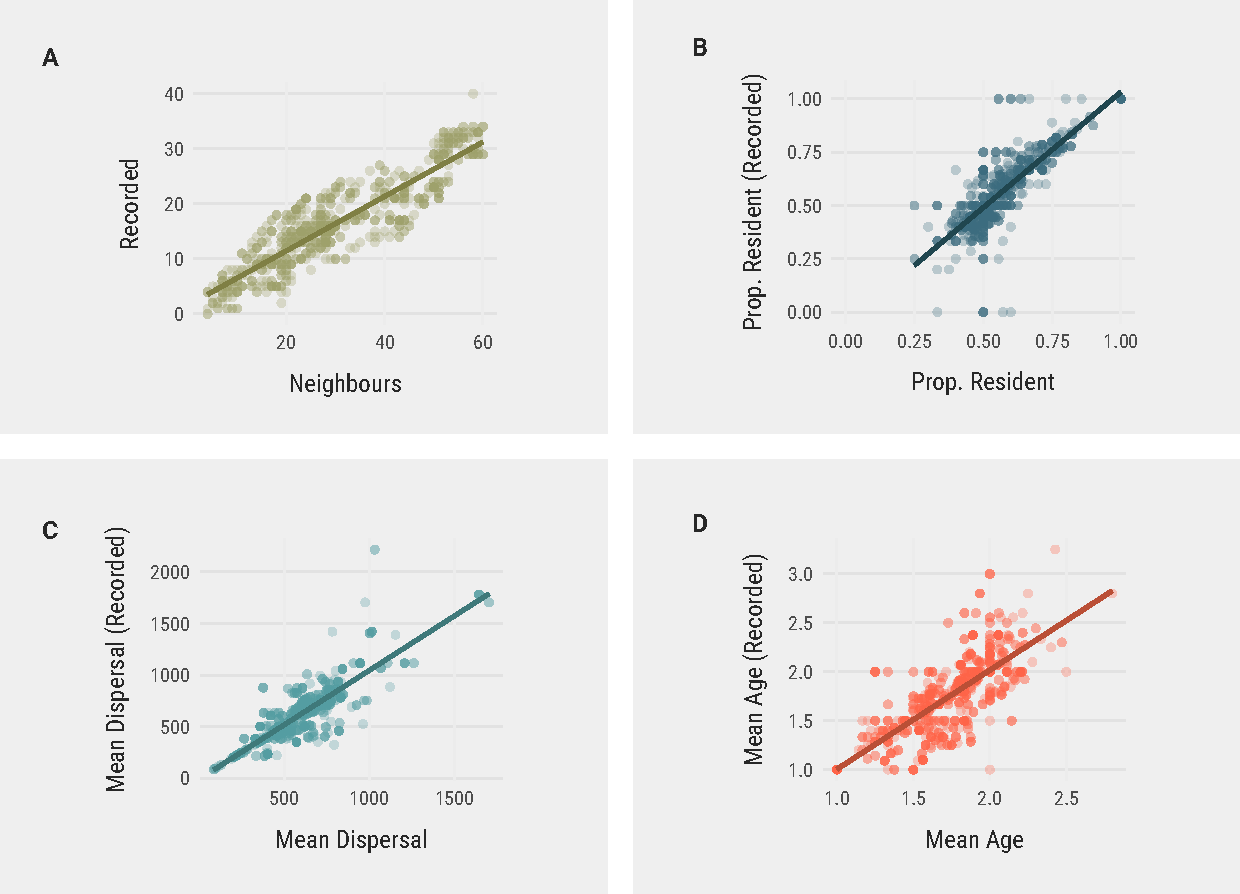
\includegraphics[width=\linewidth]{figures/chapter_4/supp_neighbourhood_sampling.pdf}
    \mycaption{Demographic characteristics of recorded birds compared to those of all birds in the neighbourhood}{
        Comparison between the actual neighbourhood properties and neighbourhood properties estimated from birds for which we have song recordings.
    (A) Neighbourhood size (number of individuals) and number of individuals for which we have song recordings in that same neighbourhood.
    (B) Proportion of resident birds calculated from monitoring data and only from those birds with song recordings. Residents are birds that were ringed as nestlings in the population.
    (C) Mean dispersal distance of the birds in a neighbourhood calculated from monitoring data and only from birds with song recordings.
    (D) Mean age of birds in a neighbourhood calculated from monitoring data and only from birds with song recordings.
    }
    \label{fig:supp_neighbourhood_sampling}
\end{figure}


\begin{figure}[tbp]
    \centering
    \includegraphics[width=\linewidth]{figures/chapter_4/supp_demo_variables.pdf}
    \mycaption{Spatial distribution of the neighbourhood-level predictor variables in the study}{
    (A) Mean natal dispersal distance, or the mean distance between the natal nest box and the breeding site for all birds in the neighbourhood.
    (B) Proportion of immigrant birds in the neighbourhood.
    (C) Mean age of birds in the neighbourhood.
    (D) Individual turnover, or the proportion of birds that were not already in a neighbourhood in the preceding year.
    }
    \label{fig:supp_demo_variables}
\end{figure}

\begin{figure}[tbp]
    \centering
    \includegraphics[width=\linewidth]{figures/chapter_4/supp_song_typle_clusters.pdf}
    \mycaption{Examples of song type clusters in the study population}
    {
Colours and connected lines represent the same song type cluster sung by different birds. Some song types are sung by many birds, while others are unique to a single bird. The clustering process is based on song similarity derived from a deep metric learning model and a manual categorization process following McGregor and Krebs \autocite{mcgregor1982b}.
    }
    \label{fig:supp_song_typle_clusters}
\end{figure}


\begin{figure}[tbp]
    \centering
    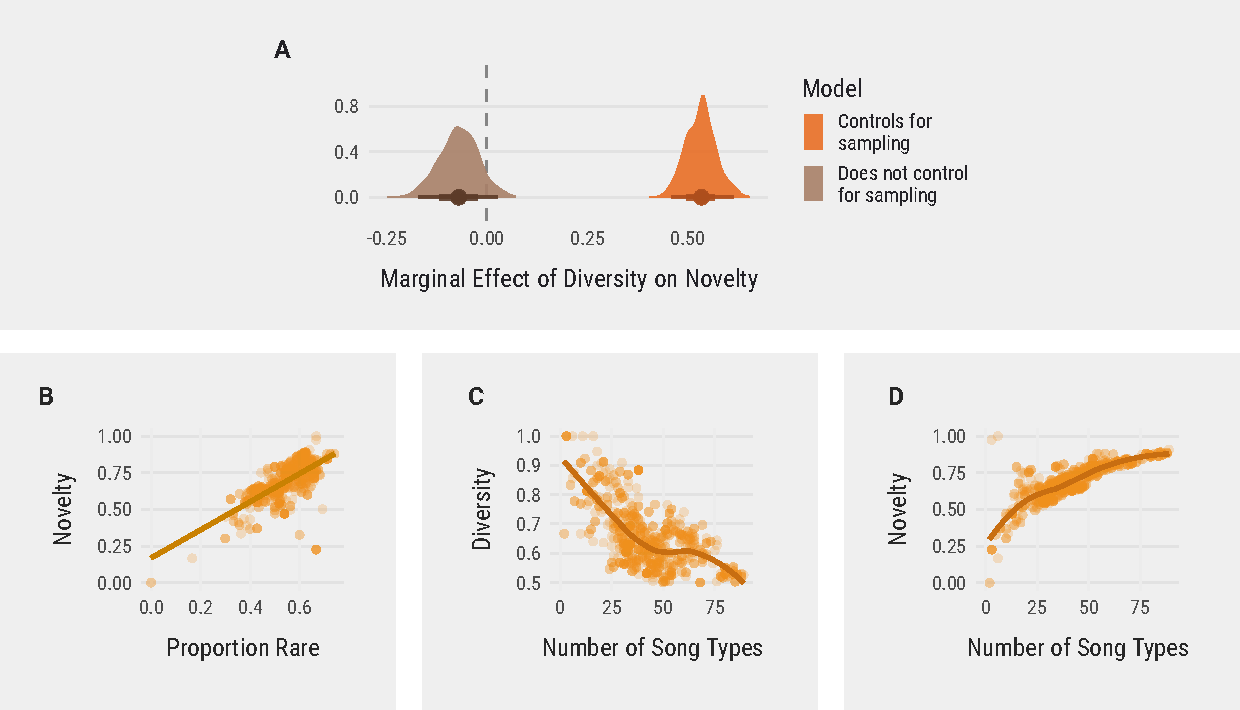
\includegraphics[width=\linewidth]{figures/chapter_4/supp_song_sampling.pdf}
    \mycaption{Estimates of cultural outcomes depend on the size of the neighbourhood repertoire}
    {
        (A) Marginal effect of diversity---which describes the proportion of distinct songs in a neighbourhood---on uniqueness, that is, how rare, on average, the songs of the birds in a neighbourhood are in the popualtion. These two ways of characterizing cultural diversity are anti-correlated in our study site due to the effect of sampling: more frequent songs are sampled more readily, causing larger sample sizes (neighbourhoods with more birds and therefore songs) to yield lower average estimates of diversity (C) and higher average estimates of uniqueness (D), in a nonlinear manner. Once this is adjusted for, which we do by including GAM terms capturing neighbourhood song density or number of birds, diversity and uniqueness are positively correlated, as expected. (B) Our measure of cultural uniqueness (y-axis) has the advantages of being continuous and not using an arbitrary cut-off, but is nonetheless correlated with definitions traditionally used in the literature, such as 'songs shared by fewer than 4 birds” \autocite{mcgregor1982b}, here on the x-axis.}
    \label{fig:supp_song_sampling}
\end{figure}

\begin{figure}[tbp]
    \centering
    \includegraphics[width=\linewidth]{figures/chapter_4/supp_cultural_variables.pdf}
    \mycaption{Spatial distribution of the neighbourhood-level cultural variables in the study}
    {
        (A) Relative cultural diversity ('diversity'): the ratio of distinct song types recorded in a neighbourhood to the total number of songs recorded in that neighbourhood. Higher values indicate that there are more distinct song types in the neighbourhood relative to its total song output.
        (B) Uniqueness index: the complement of the logarithm of the mean population-wide frequency of the song types present in a neighbourhood. Higher values indicate that the songs in the neighbourhood are on average less common in the population.
        (C) Cultural turnover: the proportion of distinct song types recorded in a neighbourhood that were not present in the previous year. Higher values indicate that the neighbourhood's song repertoire has changed more from one year to the next.
        As described in \autoref{fig:supp_song_sampling}, (A) and (B) are anti-correlated due to the effect of sampling, but once this is adjusted for, neighbourhoods with more cultural diversity also tend to have more distinct songs, as expected.
        }
    \label{fig:supp_cultural_variables}
\end{figure}


\begin{figure}[tbp]
    \centering
    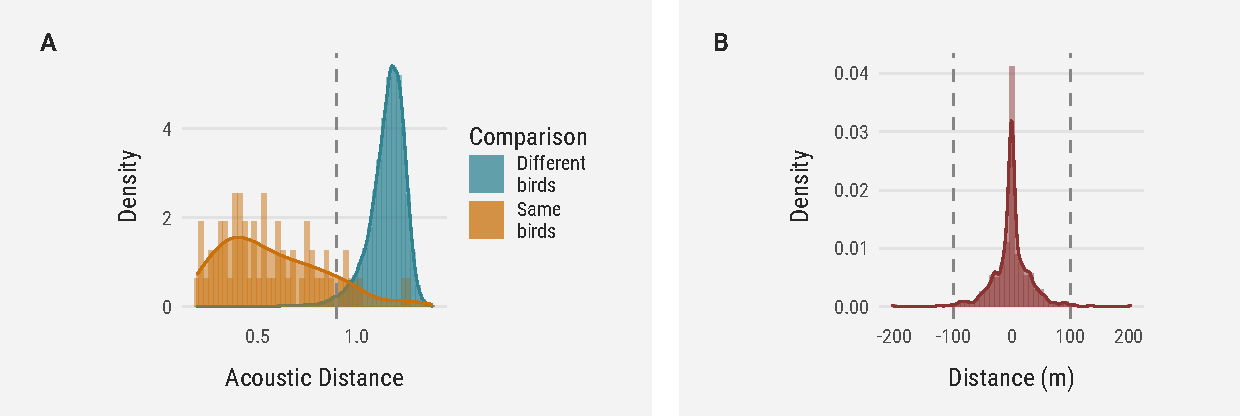
\includegraphics[width=\linewidth]{figures/chapter_4/supp_acoustic_distance_threshold.pdf}
    \mycaption{Thresholds for re-identifying individual birds based on their songs}{
    We used conservative criteria to infer when two repertoires belong to the same bird. Acoustic similarity: A minimum of two matching songs must be more similar than the 0.025 quantile of the distance distribution (an acoustic distance of 0.9). Spatial proximity: The bird must be no more than 100 meters apart from the reference bird.
    Accuracy of the method: Using only acoustic distance: 0.3\% error rate (34 out of 11,359 unique comparisons). Using acoustic distance and spatial constraint: 0.04\% error rate (4 out of 11,359 comparisons). These error rates were calculated using only ground truth data from physically re-identified birds across years.

     (A) Distribution of acoustic distances. Orange: Same song type sung by the same known bird in different years. Blue: Minimum pairwise distance between different birds and years. Vertical dashed line: x-intercept at 0.9, representing the acoustic distance threshold
 
     (B) Distribution of distance changes between breeding sites for birds that bred more than once. Demonstrates high nest site fidelity in adult birds, which we use as an additional constraint for re-identification. Vertical dashed lines: 100 m threshold.
 }
    \label{fig:supp_acoustic_distance_threshold}
\end{figure}


\begin{figure}[tbp]
    \centering
    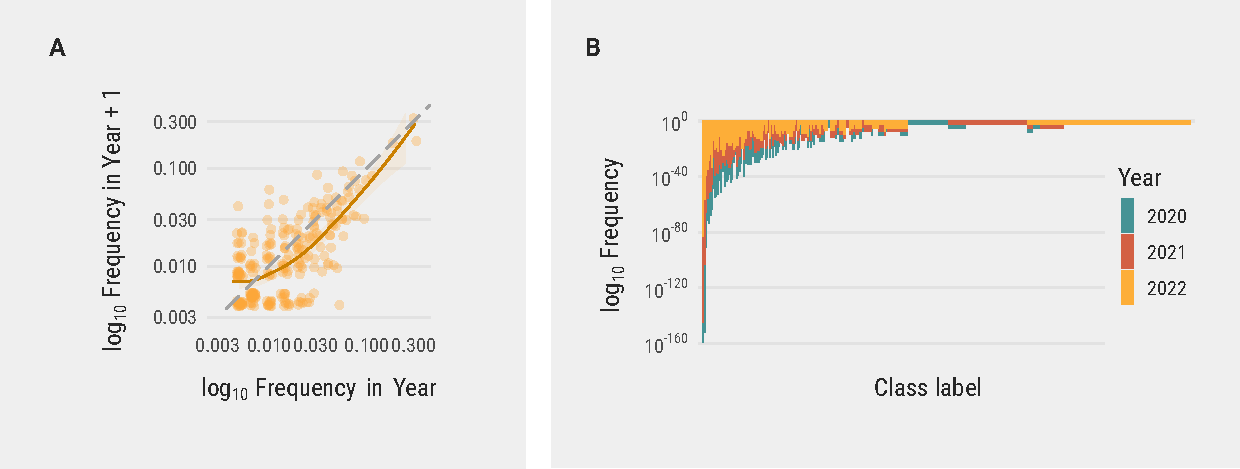
\includegraphics[width=\linewidth]{figures/chapter_4/supp_song_frequencies.pdf}
    \mycaption{
        Song frequencies and their relationship with abundance in the following year}{
        (A) The abundance of a song type in a year predicts its abundance in the following year, with higher stochasticity around rare songs. (B) Histogram showing the frequency of individual song types in the study.
    }
    \label{fig:supp_song_frequencies}
\end{figure}

\begin{figure}[tbp]
    \centering
    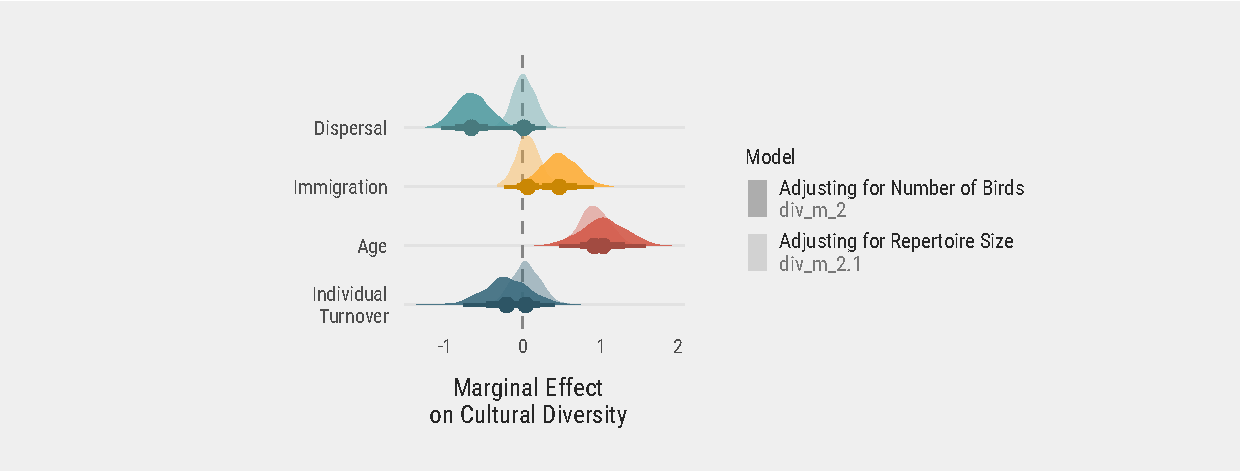
\includegraphics[width=\linewidth]{figures/chapter_4/supp_absolute_cultural_diversity.pdf}
    \mycaption{Effect of demographic variation on absolute cultural diversity within neighbourhoods}{
        To explore how the number of individuals and their repertoire sizes within a neighbourhood affect the total number of distinct song types recorded within a neighbourhood (as opposed to the relative diversity reported in \autoref{c4_fig:diversity}), we fit two models: one adjusting for the nonlinear effect of the number of individuals (higher opacity fill, corresponding to model \textit{div\_m\_2}), and a second adjusting for the nonlinear effect of the number of song types, including repeated variants (lower opacity fill, \textit{div\_m\_2.1}). See \autoref{table:model_info} for full model specifications.
    }
    \label{fig:supp_absolute_cultural_diversity}
\end{figure}

\begin{figure}[tbp]
    \centering
    \includegraphics[width=\linewidth]{figures/chapter_4/supp_dispersal_simulation.pdf}
    \mycaption{Simulation of the effect of natal dispersal on repertoire uniqueness}
    {
        We simulate the relationship between pre-breeding bird movement and the uniqueness of songs in their repertoires  (relative to the population). We initialize 200 birds in a 1500 x 1500 square, each capable of singing 4 songs selected from
        a pool of 200 song types. Birds do not initially move. New birds are born and move based on a log-normal distribution parametrized to represent realistic dispersal behaviour in our population. Each bird can learn the songs it hears within a 200 m radius as it moves. At the end of their movement, a bird's crystallized repertoire is determined by its learning mechanism: (A) random learning of songs, (B) linearly frequency-dependent learning, (C) positively frequency-dependent learning, or (D) learn the most popular songs (strong conformism). The simulation is repeated $n$ times per learning strategy, and we record the average uniqueness of songs in each bird's repertoire, which is a transformation of the average frequency of the bird's songs, as well as the distance that each bird has moved. The results show that the relationship between dispersal and repertoire uniqueness depends on the learning mechanism, and that the effect of dispersal detected in our study might be expected to arise if being exposed to a larger number of songs influences learning in a nonlinear frequency-dependent manner.
    }
    \label{fig:supp_dispersal_simulation}
\end{figure}


\begin{figure}[tbp]
    \centering
    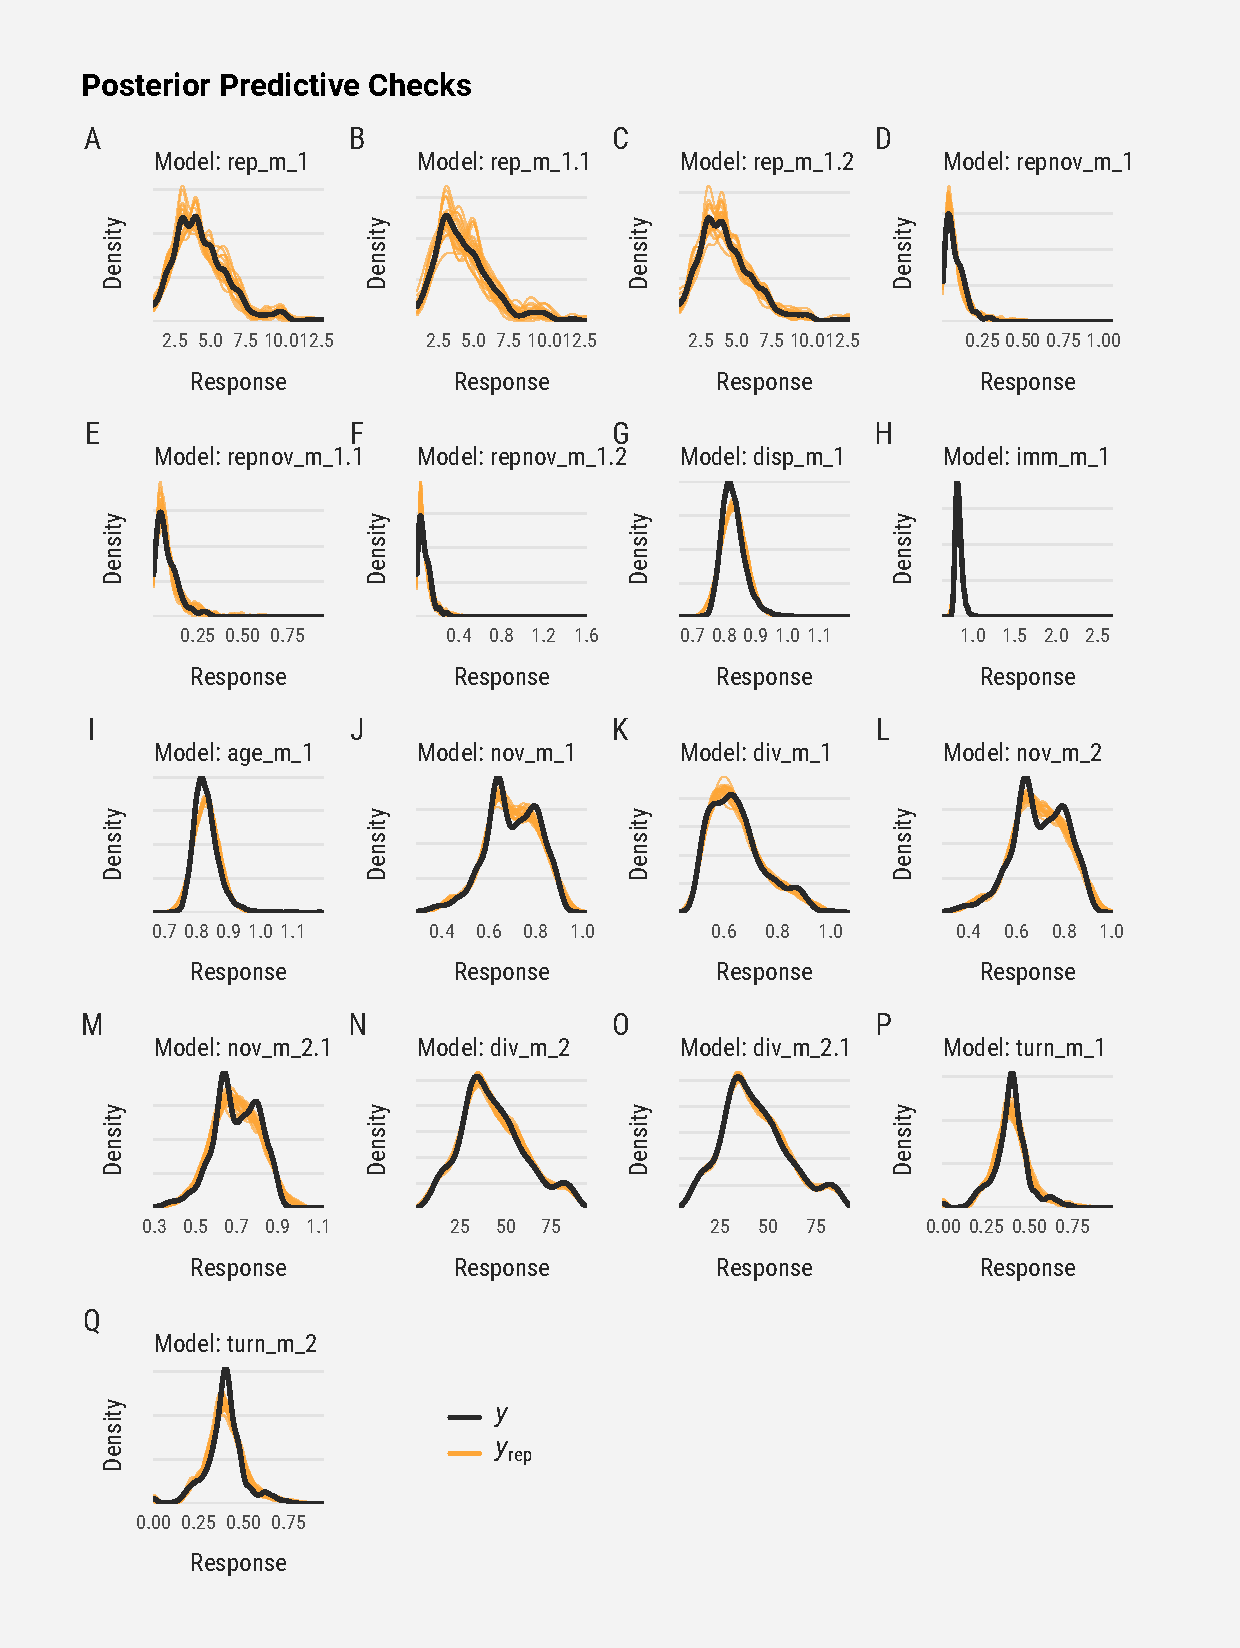
\includegraphics[width=\linewidth]{figures/chapter_4/supp_pp_checks.pdf}
    \mycaption{
        Posterior predictive checks for the main models in the study}{Comparing simulations from the posterior predictive distribution $y^{rep}$ (thin orange lines) with the outcome $y$ (black lines) using Kernel density estimates. The posterior predictive distribution is a distribution of possible outcomes of the model given the data and the model parameters, here used to check the fit of the model to the data.
    }
    \label{fig:supp_pp_checks}
\end{figure}


\end{document} 